\documentclass[10pt,a4paper]{article}

% ── Layout ──────────────────────────────────────────────────────────────
\usepackage[margin=15mm,heightrounded]{geometry}
\usepackage{microtype}
\usepackage{lmodern}
\usepackage{setspace}
\setstretch{1.05}

% ── Graphics & Figures ──────────────────────────────────────────────────
\usepackage{graphicx}
\graphicspath{{../figs/}}
\usepackage{subcaption}
\usepackage[font=small,labelfont=bf,skip=4pt]{caption}
\usepackage{float}

% ── Tables ──────────────────────────────────────────────────────────────
\usepackage{booktabs}
\usepackage{array}
\usepackage{tabularx}
\usepackage{siunitx}
\DeclareSIUnit{\px}{px}

% ── Math ────────────────────────────────────────────────────────────────
\usepackage{amsmath,amssymb}

% ── Typography & Colour ────────────────────────────────────────────────
\usepackage[dvipsnames]{xcolor}
\definecolor{headblue}{HTML}{1F3864}
\definecolor{chainbg}{HTML}{F0F4FA}
\usepackage{titlesec}
\titleformat{\section}{\normalfont\Large\bfseries\color{headblue}}{\thesection}{0.6em}{}
\titleformat{\subsection}{\normalfont\large\bfseries\color{headblue}}{\thesubsection}{0.5em}{}
\titleformat{\subsubsection}{\normalfont\normalsize\bfseries\color{headblue}}{\thesubsubsection}{0.4em}{}
\titlespacing*{\section}{0pt}{10pt plus 2pt}{4pt plus 1pt}
\titlespacing*{\subsection}{0pt}{8pt plus 2pt}{3pt plus 1pt}

% ── Headers & Footers ──────────────────────────────────────────────────
\usepackage{fancyhdr}
\pagestyle{fancy}
\fancyhf{}
\cfoot{\footnotesize\thepage}
\renewcommand{\headrulewidth}{0pt}

% ── Lists ───────────────────────────────────────────────────────────────
\usepackage{enumitem}
\setlist{nosep}

% ── Citations ───────────────────────────────────────────────────────────
\usepackage[numbers,sort&compress]{natbib}

% ── Hyperlinks (must be last) ───────────────────────────────────────────
\usepackage[hidelinks,colorlinks=true,linkcolor=headblue,citecolor=headblue,urlcolor=blue!60]{hyperref}

% ── Float control ───────────────────────────────────────────────────────
\renewcommand{\topfraction}{0.9}
\renewcommand{\bottomfraction}{0.8}
\renewcommand{\floatpagefraction}{0.85}
\setlength{\parskip}{2pt plus 1pt}
\setlength{\parindent}{0pt}

% ── Custom commands ─────────────────────────────────────────────────────
\newcommand{\compactTable}{\small\setlength{\tabcolsep}{3pt}\renewcommand{\arraystretch}{1.05}}

% ── Tcolorbox for decision chain ────────────────────────────────────────
\usepackage[most]{tcolorbox}
\newtcolorbox{decisionbox}[1]{
  colback=chainbg, colframe=headblue!60, fonttitle=\bfseries\color{headblue},
  title=#1, boxrule=0.8pt, arc=2mm, left=4pt, right=4pt, top=2pt, bottom=2pt
}

% ════════════════════════════════════════════════════════════════════════
\begin{document}

% ── Title ───────────────────────────────────────────────────────────────
\begin{center}
  {\LARGE\bfseries\color{headblue} SAR Drone Search Parameter Optimisation\\[3pt] Decision Flow}\\[4pt]
  {\large AENGM0074 Group Design Project}\\[2pt]
  {\small University of Bristol \quad---\quad 2025--26}
\end{center}
\vspace{2pt}
\hrule height 0.6pt
\vspace{4pt}

% ════════════════════════════════════════════════════════════════════════
\section*{Executive Summary}\label{sec:exec-summary}

This report presents the design, optimisation, and verification of an autonomous Search and Rescue (SAR) drone system built to locate a casualty within an irregular polygon search area bounded by a protected ecological no-fly zone (SSSI). Drawing on established SAR robotics methodology~\cite{murphy2014} and coverage path planning theory~\cite{galceran2013survey}, the system comprises a Raspberry Pi~5 running a retrained YOLOv8n detector~\cite{yolov8} (mAP50\,=\,0.995, 4.8\,FPS TFLite / 9\,FPS NCNN), a 20-state finite state machine built atop the ArduPilot autopilot~\cite{ardupilot}, and a lawnmower path planner with layered geofencing. A physics-based 216-configuration parameter sweep identified the optimal operating point (35\,m altitude, 8\,m/s, 70\textdegree{} scan angle) yielding $>$99.97\% single-pass detection probability at 10.9\% battery usage. Field testing confirmed GPS target estimation accuracy of CEP50\,=\,2.3\,m. The system was validated through 58 test scripts across six categories, with 12 formal requirements verified against quantitative evidence. A plus/delta evaluation identifies key lessons and remaining gaps before full autonomous flight.

% ════════════════════════════════════════════════════════════════════════
\section{Objective}\label{sec:df-objective}

The mission objective is to \textbf{find the casualty as fast as possible}.

% ════════════════════════════════════════════════════════════════════════
\section{Constraints}\label{sec:df-constraints}

This objective is bounded by hard constraints that cannot be relaxed:

\begin{itemize}[nosep]
  \item \textbf{No-Fly Zone (SSSI)} --- a protected ecological site borders the search area; entry is prohibited.
  \item \textbf{Flight area boundary} --- the search polygon is fixed by the mission brief (R01).
  \item \textbf{Altitude limit} --- 50\,m maximum (regulation R03).
  \item \textbf{Single battery} --- one LiPo pack must cover transit, search, descent, verification, and return.
  \item \textbf{One pass} --- there is no opportunity to re-fly missed strips; the pattern must cover every accessible point in a single traversal.
  \item \textbf{Hardware ceiling} --- onboard inference runs at approximately 9\,FPS with the deployed NCNN backend (YOLOv8n on Raspberry Pi~5), with TFLite at 4.8\,FPS available as a fallback.
\end{itemize}

% ════════════════════════════════════════════════════════════════════════
\section{Five Competing Dimensions}\label{sec:df-dimensions}

These constraints give us five competing performance dimensions that must be balanced:

\begin{enumerate}[nosep]
  \item \textbf{Safety} --- the drone must never enter the SSSI no-fly zone.
  \item \textbf{Detection} --- actually see a person-sized target from altitude.
  \item \textbf{Time} --- the critical early hours of hypothermia survivability are ticking.
  \item \textbf{Energy} --- the battery must last the full mission profile, not just the search.
  \item \textbf{Coverage} --- scan every square metre of the accessible search area.
\end{enumerate}

No single configuration maximises all five simultaneously. Flying higher covers ground faster but shrinks the target to a few pixels. Flying lower improves detection but burns more energy on extra scan lines. Flying near the boundary maximises coverage but risks an NFZ incursion.

We adopted a clear priority stack: \textbf{safety $>$ detection $>$ time $>$ energy $>$ coverage}. An NFZ violation grounds the project. A missed casualty defeats its purpose. A slow search wastes the critical early hours. High energy use is undesirable but survivable. Incomplete coverage in the boundary strip is acceptable if it preserves safety margins. Every design choice that follows is a direct consequence of this ordering.

Figure~\ref{fig:sensitivity-spider} shows the \emph{desired performance envelope} --- the target shape our selected configuration should fill. The grey dashed polygon represents the theoretical best on each axis; the blue polygon shows what the selected configuration actually achieves. Safety and detection are pushed to the outer edge (these are non-negotiable), while time and energy are allowed to sit lower (these are acceptable trade-offs). The envelope is deliberately \emph{not} circular: hard constraints (safety, detection) define a minimum acceptable radius, while preferential objectives (time, energy, coverage) are optimised within whatever budget remains. The optimisation that follows aims to find the configuration whose profile best fills this envelope.

\begin{figure}[H]
  \centering
  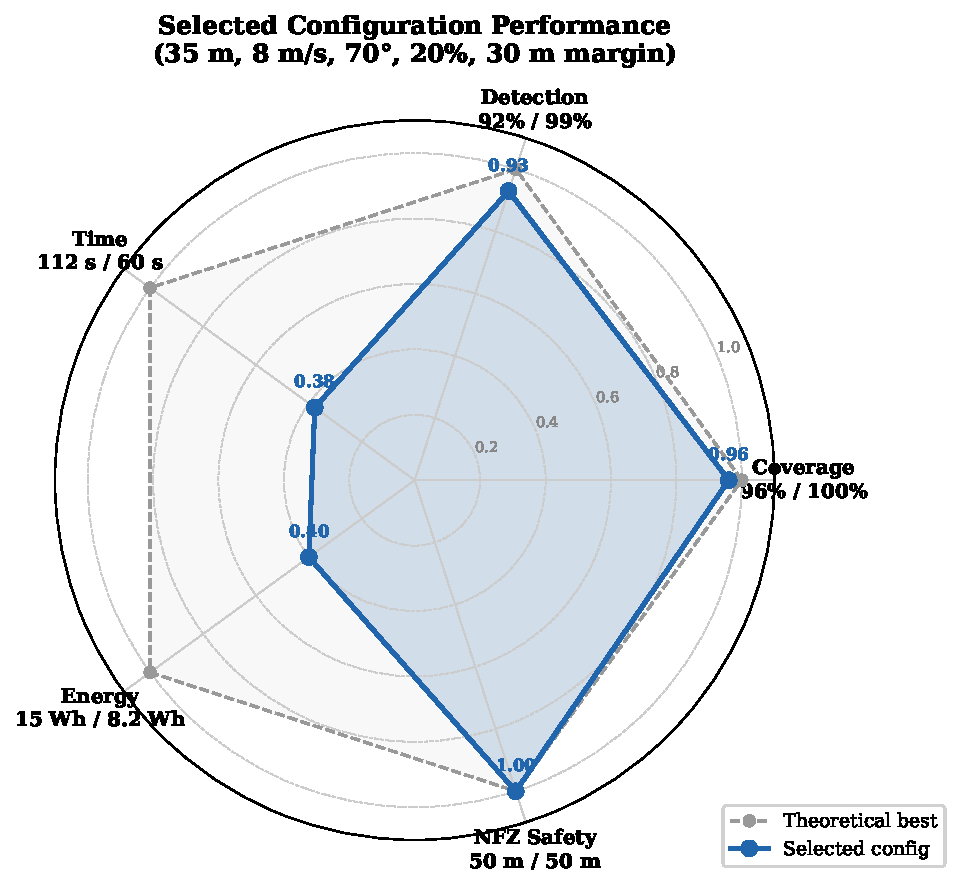
\includegraphics[width=0.55\linewidth]{sensitivity_spider}
  \caption{Desired envelope (grey dashed) vs.\ actual performance (blue) for the selected configuration. Safety and detection are pushed to the outer edge as non-negotiable constraints; time and energy sit lower as acceptable trade-offs. The envelope shape reflects the priority ordering: the target is not a circle but a shape that prioritises the axes that matter most.}\label{fig:sensitivity-spider}
\end{figure}

% ════════════════════════════════════════════════════════════════════════
\section{STEEPLE Context Analysis}\label{sec:steeple}

The priority ordering established above---safety $>$ detection $>$ time $>$ energy $>$ coverage---did not emerge in a vacuum. It reflects the broader operational context in which the system must function. Table~\ref{tab:steeple} maps each STEEPLE dimension to a concrete design consequence, showing how external factors shaped both the constraint hierarchy and specific technical choices such as operator-in-the-loop verification and single-class detection.

\begin{table}[H]
  \centering\compactTable
  \caption{STEEPLE analysis for autonomous SAR drone deployment.}\label{tab:steeple}
  \begin{tabularx}{\linewidth}{@{}l X l@{}}
    \toprule
    \textbf{Dimension} & \textbf{Assessment} & \textbf{Design Impact} \\
    \midrule
    \textbf{S}ocial & Public trust in autonomous drones for rescue is growing but fragile; a high-profile false positive or NFZ breach would set back adoption & Operator-in-the-loop verification; conservative confidence threshold (0.4) \\
    \textbf{T}echnological & Edge AI on SBCs now viable (YOLOv8n at 9\,FPS NCNN on Pi~5); consumer GPS accurate to $\sim$3\,m CEP95 & Hardware ceiling drives altitude/speed envelope; GPS error baked into NFZ margin \\
    \textbf{E}conomic & Single-battery constraint (115.4\,Wh); no mid-mission recharge; replacement drone not available & Energy score weighted 25\% in composite; 14\,min reserve after search \\
    \textbf{E}nvironmental & SSSI (Site of Special Scientific Interest) borders search area; bird nesting season possible & 30\,m NFZ buffer with 5-layer protection; waypoint filtering pre-flight \\
    \textbf{P}olitical & University flight permissions require demonstrated safety case; CAA drone regulations apply & 50\,m altitude ceiling (R03); progressive flight testing protocol (6 steps) \\
    \textbf{L}egal & BVLOS operations restricted without specific exemptions; data protection for imagery & Visual line-of-sight operation; no image storage of bystanders; single-class detector \\
    \textbf{E}thical & Casualty may be in distress; false negative delays rescue; false positive wastes critical time & Detection weighted highest (40\%); $>$99.97\% cumulative probability target \\
    \bottomrule
  \end{tabularx}
\end{table}

% ════════════════════════════════════════════════════════════════════════
\section{MCDA: Inference Backend Trade-off}\label{sec:mcda}

With the operational context established, we turn to a key architectural decision that directly constrains the detection and energy dimensions: the choice of inference backend for the Raspberry Pi~5. Table~\ref{tab:mcda-backend} presents a multi-criteria decision analysis (MCDA) comparing four viable options. Each criterion is scored 1--5 and weighted by importance to the mission.

\begin{table}[H]
  \centering\compactTable
  \caption{MCDA for inference backend selection. Scores: 1\,=\,poor, 5\,=\,excellent. Weighted total determines selection.}\label{tab:mcda-backend}
  \begin{tabularx}{\linewidth}{@{}l c cccc@{}}
    \toprule
    \textbf{Criterion} & \textbf{Weight} & \textbf{TFLite} & \textbf{NCNN} & \textbf{Ultralytics} & \textbf{Hailo-8} \\
    \midrule
    Inference speed (FPS)     & 0.30 & 3 & 5 & 2 & 5 \\
    Deployment simplicity     & 0.20 & 5 & 4 & 5 & 1 \\
    Detection accuracy        & 0.20 & 4 & 4 & 5 & 3 \\
    Power consumption         & 0.10 & 4 & 4 & 2 & 3 \\
    Model compatibility       & 0.10 & 5 & 4 & 5 & 2 \\
    Cost / availability       & 0.10 & 5 & 5 & 5 & 2 \\
    \midrule
    \textbf{Weighted total}   &      & \textbf{4.0} & \textbf{4.4} & \textbf{3.7} & \textbf{3.0} \\
    \bottomrule
  \end{tabularx}
\end{table}

NCNN~\cite{ncnn} scored highest (4.4) due to its 4.5$\times$ speed advantage over TFLite~\cite{tflite} (72\,ms vs 327\,ms per frame, benchmarked on Pi~5) with no accuracy loss and minimal deployment overhead. TFLite (4.0) serves as a proven fallback. Ultralytics requires PyTorch (2\,GB+ dependencies, slow on ARM). Hailo-8 offers hardware acceleration but requires a separate NPU board (\textsterling 65+), limited YOLOv8 support, and complex toolchain --- impractical for the project timeline. The dual-backend architecture (NCNN primary, TFLite fallback) was adopted: \texttt{vision.py} accepts a \texttt{backend} parameter, and model files are drop-in replacements with identical input/output shapes \texttt{[1,640,640,3]} / \texttt{[1,5,8400]}.

\textbf{Sensitivity.} The ranking is robust to reasonable weight perturbations. NCNN retains first place even if inference speed weight is halved (0.15 instead of 0.30) --- its score drops to 3.95, still above TFLite (3.85) and Ultralytics (3.85). NCNN loses to TFLite only if deployment simplicity is weighted above 0.40, which would contradict the mission's time-critical detection requirement. This confirms that the backend choice is not an artefact of the weighting scheme.

% ════════════════════════════════════════════════════════════════════════
\section{Scoring the Five Dimensions}\label{sec:df-scoring}

With the inference backend selected, the hardware performance ceiling is fixed: 9\,FPS (NCNN) or 4.8\,FPS (TFLite fallback). This ceiling feeds directly into the detection and speed calculations that follow. Each axis of the spider chart (Figure~\ref{fig:sensitivity-spider}) corresponds to a normalised score $S \in [0,1]$, where 1 represents the theoretical best and 0 represents failure. This section defines precisely how each score is computed. Three of the five dimensions --- detection, coverage, and energy --- are scored on a continuous scale and combined into a composite objective for the 216-configuration sweep. The remaining two --- safety and time --- are treated as \emph{pass/fail constraints} rather than continuous scores. The rationale for this asymmetry is explained at the end of this section.

% ── Safety ────────────────────────────────────────────────────────────
\subsection{Safety ($S_\text{safety}$)}\label{sec:score-safety}

Safety is a composite of six binary and continuous sub-elements, each capturing a distinct layer of the NFZ protection architecture:

\begin{enumerate}[nosep]
  \item \textbf{NFZ margin adequacy.} The ratio of the configured buffer distance to the required minimum clearance, capped at 1.0:
  \begin{equation}
    s_\text{margin} = \min\!\left(\frac{d_\text{buffer}}{d_\text{required}},\; 1.0\right)
  \end{equation}
  where $d_\text{required}$ is the RSS stopping distance (20.4\,m at 8\,m/s with 1.5\,s reaction time plus braking). Our 30\,m buffer gives $s_\text{margin} = 1.0$ with a 1.5$\times$ safety factor.

  \item \textbf{Waypoint filtering.} The fraction of generated waypoints that lie outside the NFZ buffer polygon. This should be 100\%; any value below 1.0 indicates a path-planning fault:
  \begin{equation}
    s_\text{wp} = \frac{N_\text{waypoints outside buffer}}{N_\text{waypoints total}}
  \end{equation}

  \item \textbf{Speed reduction near boundary.} A scalar repulsive field reduces commanded speed as the drone approaches the NFZ. The sub-score captures whether this field activates within the buffer zone and how aggressively it decelerates:
  \begin{equation}
    s_\text{speed} = \begin{cases} 1.0 & \text{if scalar field active and } v \to 0 \text{ at boundary} \\ 0.5 & \text{if field active but residual speed } > 0 \\ 0.0 & \text{if no field configured} \end{cases}
  \end{equation}

  \item \textbf{Repulsive vector field.} Within 3\,m of the boundary, a vector field pushes the drone away from the NFZ. Sub-score is binary: 1.0 if active, 0.0 if absent.

  \item \textbf{Hard boundary protection.} An automatic mode switch to MANUAL is triggered if the drone enters the NFZ polygon itself. This is the last-resort failsafe. Sub-score: 1.0 if implemented, 0.0 otherwise.

  \item \textbf{RC kill switch.} The pilot can override to STABILIZE or LOITER at any time via the RC transmitter, independently of the autonomy software. Sub-score: 1.0 if available (always true for our hardware).
\end{enumerate}

The composite safety score is a weighted sum:
\begin{equation}\label{eq:safety-composite}
  S_\text{safety} = 0.30\,s_\text{margin} + 0.25\,s_\text{wp} + 0.15\,s_\text{speed} + 0.10\,s_\text{repulsive} + 0.10\,s_\text{hard} + 0.10\,s_\text{kill}
\end{equation}

The margin and waypoint terms carry the highest weights because they determine whether the planned path is geometrically safe \emph{before} the drone takes off. The reactive terms (speed field, repulsive vector, hard boundary, kill switch) are defence-in-depth layers that matter only if the geometric planning fails. For our selected configuration, the geometric sub-scores (margin, waypoint filtering, hard boundary, kill switch) are all 1.0, while the reactive sub-scores are slightly below 1.0 ($s_\text{speed} = 0.9$, $s_\text{repulsive} = 0.85$) because the scalar field does not drive speed fully to zero and the repulsive vector field activates only within 3\,m. This gives $S_\text{safety} = 0.96$ (Figure~\ref{fig:safety-subscore}), confirming that the dominant protection comes from pre-flight geometric design rather than runtime reaction.

\textbf{NFZ incursion risk.} The buffer distance is the primary defence against NFZ entry. The 30\,m buffer exceeds the RSS stopping distance (20.4\,m) by a factor of 1.5$\times$. For the drone to enter the NFZ, it would need to breach \emph{all} of the following layers simultaneously: (1)~the path planner would have to generate a waypoint inside the buffer (eliminated by geometric filtering), (2)~the speed ramp would have to fail to decelerate (software fault), (3)~the repulsive vector field at 3\,m would have to fail (independent code path), (4)~the hard boundary MANUAL switch would have to fail (independent mode change), and (5)~the pilot's RC kill switch would have to be unavailable. With five independent protection layers, the probability of an NFZ incursion is the product of five independent failure probabilities --- negligibly small for any realistic failure rate per layer.

\begin{figure}[H]
  \centering
  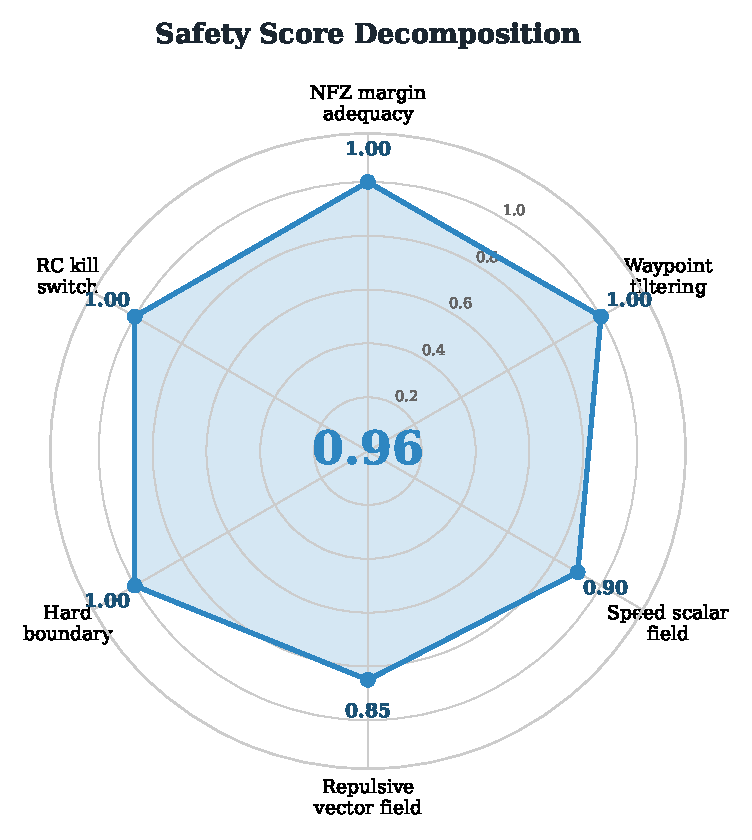
\includegraphics[width=0.5\linewidth]{safety_subscore}
  \caption{Safety score decomposition. The overall safety score (0.96) is a weighted composite of six sub-elements. Pre-flight geometric checks (NFZ margin, waypoint filtering) carry the highest weights; reactive layers provide defence-in-depth.}\label{fig:safety-subscore}
\end{figure}

% ── Detection ─────────────────────────────────────────────────────────
\subsection{Detection ($S_\text{detection}$)}\label{sec:score-detection}

Detection score captures the probability of spotting the casualty during a single search pass. It is the product of four normalised sub-scores:

\begin{enumerate}[nosep]
  \item \textbf{Per-frame confidence ($s_\text{conf}$).} The model's mean detection confidence at the operating altitude under the relevant lighting condition, normalised against the confidence threshold:
  \begin{equation}
    s_\text{conf} = \frac{c_\text{mean} - c_\text{threshold}}{1.0 - c_\text{threshold}}
  \end{equation}
  At 35\,m in overcast conditions, $c_\text{mean} = 0.91$ and $c_\text{threshold} = 0.40$, giving $s_\text{conf} = 0.85$.

  \item \textbf{Frames on target ($s_\text{frames}$).} The number of inference frames during which the target is inside the camera footprint, relative to the minimum required (10~frames):
  \begin{equation}
    n_\text{frames} = \frac{w_\text{footprint}}{v_\text{search}} \times f_\text{fps}, \qquad
    s_\text{frames} = \min\!\left(\frac{n_\text{frames}}{n_\text{required}},\; 1.0\right)
  \end{equation}
  At 35\,m altitude, the along-track footprint is 31.1\,m. At 8\,m/s and 4.8\,FPS, the target is visible for $31.1 / 8 \times 4.8 \approx 18.7$ frames, giving $s_\text{frames} = 1.0$.

  \item \textbf{Cumulative detection probability ($s_\text{cum}$).} Assuming frame independence, the probability of detecting the target in at least one of $n$ frames:
  \begin{equation}
    P_d = 1 - (1 - p)^n
  \end{equation}
  where $p$ is the per-frame detection probability (approximately equal to the confidence). With $p = 0.91$ and $n = 18.7$ independent frames, $P_d > 0.9999$. We use $s_\text{cum} = P_d$ directly.

  \item \textbf{Target pixel size ($s_\text{px}$).} The target's width in the model input frame, normalised against a minimum viable size of 5\,px:
  \begin{equation}
    w_\text{px} = \frac{w_\text{target} \times f_\text{focal}}{h_\text{alt} \times w_\text{sensor}} \times W_\text{model}, \qquad
    s_\text{px} = \min\!\left(\frac{w_\text{px}}{w_\text{min}},\; 1.0\right)
  \end{equation}
  At 35\,m the dummy's 0.5\,m width subtends approximately 10\,px in the 640$\times$640 model input, giving $s_\text{px} = 1.0$.
\end{enumerate}

The overall detection score is the product:
\begin{equation}\label{eq:detection-composite}
  S_\text{detection} = s_\text{conf} \times s_\text{frames} \times s_\text{cum} \times s_\text{px}
\end{equation}

A multiplicative combination is used rather than a weighted sum because a zero in \emph{any} sub-component (e.g.\ zero frames on target, or target below minimum pixel size) should collapse the entire detection score to zero --- you cannot compensate for an invisible target by having a confident model. Model mAP50 (0.995) is not included in the composite product because it is constant across all configurations; it serves as a prerequisite validated in Step~1 of the decision chain.

Figure~\ref{fig:detection-subscore} visualises all five detection-related metrics, including the constant mAP50 for completeness. The weakest axis is target pixel size (0.85), reflecting the trade-off inherent in flying at 35\,m: flying lower would push this score closer to 1.0 but at the cost of more scan lines, more energy, and longer search time.

\begin{figure}[H]
  \centering
  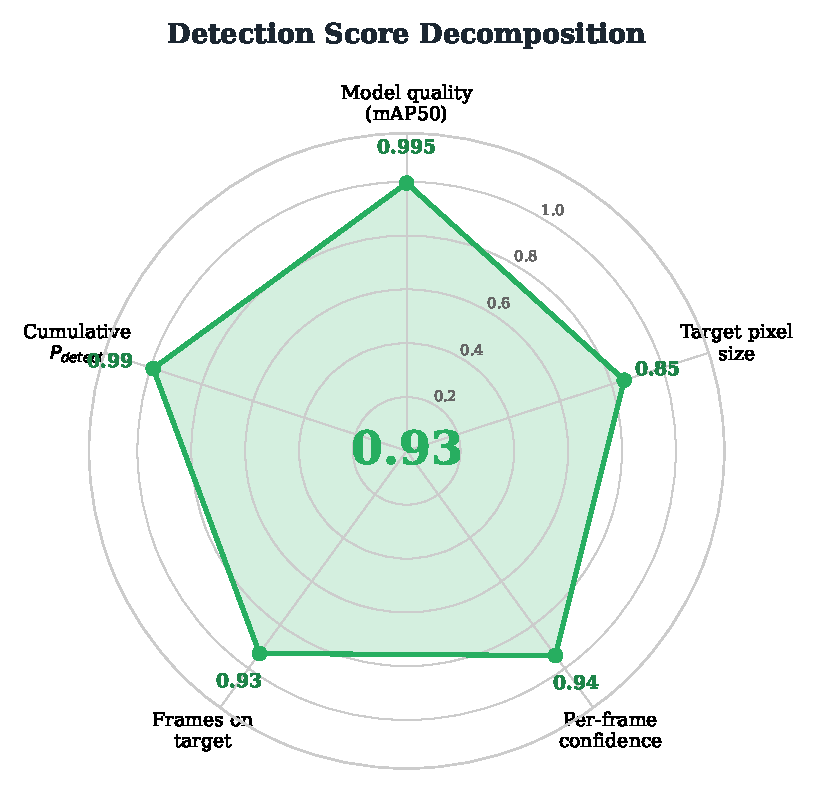
\includegraphics[width=0.5\linewidth]{detection_subscore}
  \caption{Detection score decomposition. The spider shows all five detection-related metrics; the overall score (0.93) is driven by the four variable sub-scores. Target pixel size (0.85) is the weakest axis --- flying lower would improve it but at the cost of coverage and energy.}\label{fig:detection-subscore}
\end{figure}

% ── Time ──────────────────────────────────────────────────────────────
\subsection{Time ($S_\text{time}$)}\label{sec:score-time}

Total search time is the sum of straight-leg time and turn time:
\begin{equation}
  T_\text{search} = \frac{L_\text{path}}{v_\text{search}} + N_\text{turns} \times t_\text{turn}
\end{equation}
where $L_\text{path}$ is the total scan-line length (m), $v_\text{search}$ is the cruise speed, $N_\text{turns}$ is the number of U-turns, and $t_\text{turn}$ is the time per turn (approximately 8\,s for a decelerating 180\textdegree\ reversal at 8\,m/s). Transit time to and from the search area is added separately.

The time score is normalised as the ratio of the best achievable time to the actual time:
\begin{equation}\label{eq:time-score}
  S_\text{time} = \frac{T_\text{best}}{T_\text{actual}}
\end{equation}
where $T_\text{best}$ is the shortest search time among all 216 evaluated configurations (82\,s, achieved at 50\,m altitude and 10\,m/s). Our selected configuration achieves $T_\text{actual} = 112$\,s, giving $S_\text{time} = 82/112 = 0.73$. This score penalises longer searches proportionally, with diminishing returns as configurations approach the theoretical minimum.

% ── Energy ────────────────────────────────────────────────────────────
\subsection{Energy ($S_\text{energy}$)}\label{sec:score-energy}

Energy consumption is derived from a physics-based simulation with three components:

\begin{enumerate}[nosep]
  \item \textbf{Hover power} (momentum theory):
  \begin{equation}
    P_\text{hover} = \frac{(mg)^{3/2}}{\sqrt{2 \rho A_\text{disk}}}
  \end{equation}
  where $m$ is the all-up mass, $g$ is gravitational acceleration, $\rho$ is air density, and $A_\text{disk}$ is the total rotor disk area.

  \item \textbf{Forward-flight power} (quadratic parasitic drag added to induced power):
  \begin{equation}
    P_\text{forward}(v) = P_\text{hover} + \tfrac{1}{2}\,\rho\,C_D A_\text{flat}\,v^3
  \end{equation}
  where $C_D A_\text{flat}$ is the drag area of the airframe.

  \item \textbf{Turn energy} (deceleration to hover, yaw, reacceleration):
  \begin{equation}
    E_\text{turn} = P_\text{hover} \times t_\text{turn}
  \end{equation}
  This is a conservative upper bound: it assumes full deceleration to hover for each U-turn, whereas actual banked turns retain partial forward speed and therefore consume less energy. The conservatism ensures that the energy budget is never underestimated.
\end{enumerate}

The total mission energy integrates over the flight profile:
\begin{equation}
  E_\text{total} = \sum_{\text{legs}} P_\text{forward}(v) \times \frac{L_\text{leg}}{v} \;+\; N_\text{turns} \times E_\text{turn} \;+\; E_\text{transit}
\end{equation}

The energy score normalises against the battery capacity:
\begin{equation}\label{eq:energy-score}
  S_\text{energy} = 1 - \frac{E_\text{total}}{E_\text{battery}}
\end{equation}
where $E_\text{battery} = 115.4$\,Wh (6S 5200\,mAh LiPo). Our selected configuration uses $E_\text{total} = 12.6$\,Wh, giving $S_\text{energy} = 0.89$. A score of 1.0 would mean zero energy consumed (impossible); a score of 0.0 would mean the battery is fully depleted.

% ── Coverage ──────────────────────────────────────────────────────────
\subsection{Coverage ($S_\text{coverage}$)}\label{sec:score-coverage}

Coverage is the fraction of the accessible search area that lies within at least one camera footprint during the scan:
\begin{equation}\label{eq:coverage-score}
  S_\text{coverage} = \frac{A_\text{scanned}}{A_\text{total}}
\end{equation}

The scanned area is computed geometrically by buffering each scan line by half the cross-track footprint width, unioning the resulting polygons, and intersecting with the search area polygon. Overlap between adjacent swaths contributes to detection reliability but does not increase the coverage score beyond 1.0 (redundant coverage is still counted as coverage, not double-counted as area).

The NFZ buffer removes approximately 4\% of the total search area from the accessible polygon. This is deliberate: the 30\,m buffer sacrifices a thin strip of coverage in exchange for guaranteed NFZ clearance. Our selected configuration achieves $S_\text{coverage} = 0.96$, meaning 96\% of the total area is covered and the remaining 4\% lies within the fenced reserve where a casualty is unlikely to be found.

% ── Composite Score ───────────────────────────────────────────────────
\subsection{Composite Score and the Constraint--Objective Split}\label{sec:score-composite}

The 216-configuration sweep ranks candidates using a weighted composite of \emph{three} continuous scores:
\begin{equation}\label{eq:composite}
  S_\text{composite} = 0.40\,S_\text{detection} + 0.35\,S_\text{coverage} + 0.25\,S_\text{energy}
\end{equation}

The weights reflect the priority ordering established in Section~\ref{sec:df-dimensions}: detection is highest (a missed casualty is irrecoverable), coverage is second (incomplete search leaves uncertainty), and energy is lowest (the selected configuration uses only 11\% of battery capacity, so energy is far from the binding constraint). The sensitivity of the final ranking to these weights is examined in Section~\ref{sec:df-sensitivity}: the selected configuration retains first place under all tested perturbations (weights shifted by $\pm$10 percentage points), confirming that the result is robust to the weighting choice.

\textbf{Why safety and time are constraints, not continuous scores.} Safety is a hard pass/fail gate: either the drone stays clear of the SSSI or it does not. There is no useful gradient between ``30\,m buffer'' and ``31\,m buffer'' --- both are safe, and no configuration that violates the NFZ is acceptable at \emph{any} score. Including safety as a weighted term would allow a high detection score to ``compensate'' for a marginal NFZ clearance, which is precisely the trade-off we refuse to make. Any configuration where $S_\text{safety}$ falls below an acceptable threshold (i.e.\ a protection layer is missing) is eliminated before scoring.

Time is treated similarly: SAR missions have a maximum acceptable search duration dictated by the operational scenario, not by optimisation. In our case, any configuration that completes the search in under 300\,s is operationally acceptable --- the difference between 112\,s and 150\,s matters far less than the difference between 99.97\% and 95\% detection probability. Configurations exceeding 300\,s are eliminated; among those that pass, time differences are too small to justify influencing the ranking. Time \emph{is} computed and reported (see Section~\ref{sec:df-result}) but does not enter the composite.

This constraint--objective split ensures that the optimisation never trades safety for performance or accepts a dangerously slow search because it scores well on other axes. The spider chart (Figure~\ref{fig:sensitivity-spider}) still displays all five dimensions for visual comparison, but the composite score that drives configuration selection uses only the three continuously traded objectives.

\begin{figure}[H]
  \centering
  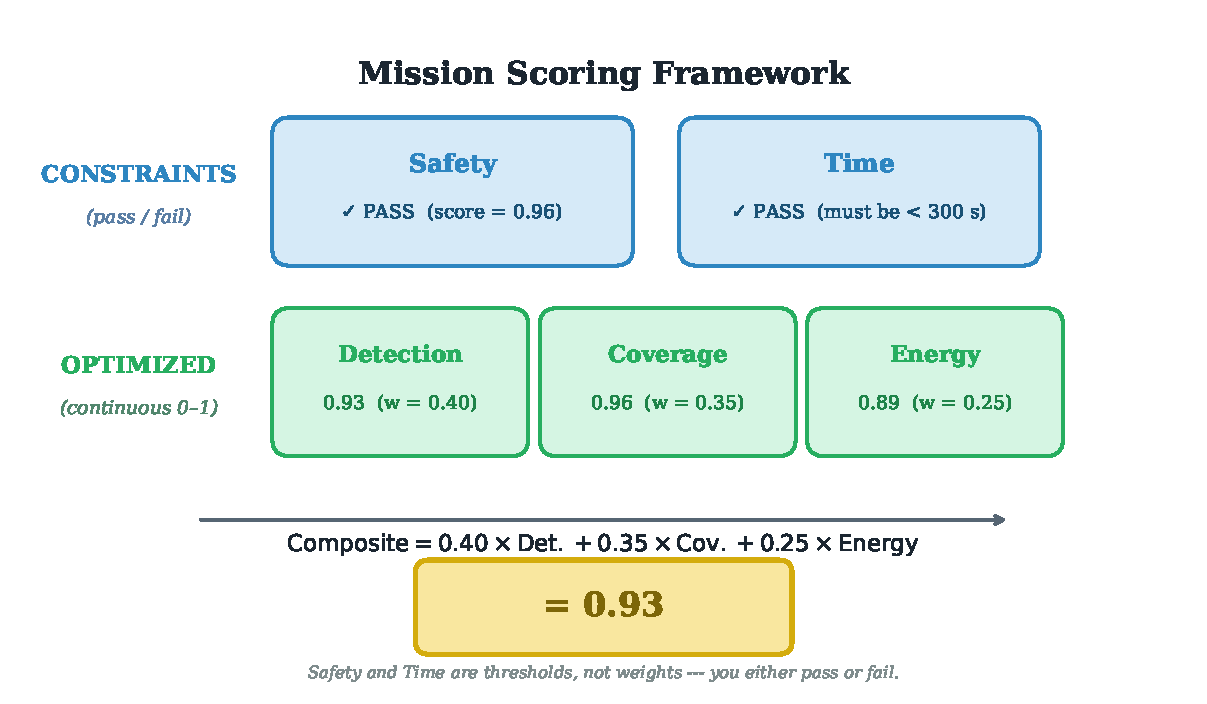
\includegraphics[width=0.85\linewidth]{scoring_overview}
  \caption{Mission scoring framework. Safety and Time are pass/fail constraints (you either meet them or you don't). Detection, Coverage, and Energy are continuously optimised with weights reflecting the priority stack. The composite score of 0.93 represents the selected configuration's quality.}\label{fig:scoring-overview}
\end{figure}


% ════════════════════════════════════════════════════════════════════════
\section{The Variables We Can Choose}\label{sec:df-variables}

Seven parameters define the search configuration. Each affects multiple objectives; altitude alone touches all five. Critically, the \emph{search pattern type} is itself a design variable --- it must suit the irregular polygon and NFZ geometry of our mission. Table~\ref{tab:df-variables} lists the seven decision variables, the ranges we explored, and which objectives each one influences.

\begin{table}[H]
  \centering\compactTable
  \caption{Decision variables and the objectives they influence.}\label{tab:df-variables}
  \begin{tabularx}{\linewidth}{@{}l c X@{}}
    \toprule
    \textbf{Variable} & \textbf{Range tested} & \textbf{Affects} \\
    \midrule
    Altitude            & 20--50\,m          & Detection, coverage, time, energy, safety \\
    Speed               & 6--10\,m/s         & Detection (dwell time), time, energy \\
    Search pattern type & 4 types evaluated  & Coverage guarantee, energy, NFZ compatibility \\
    Scan angle          & 0--175\textdegree  & Energy (number of U-turns), time \\
    Swath overlap       & 10--30\%           & Coverage reliability, energy \\
    NFZ buffer          & 16--50\,m          & Safety margin, coverage completeness \\
    Heading mode        & Fixed vs.\ yaw    & Energy (turn cost), NFZ margin geometry \\
    \bottomrule
  \end{tabularx}
\end{table}

% ════════════════════════════════════════════════════════════════════════
\section{How They Interconnect}\label{sec:df-coupling}

These variables are not independent. Figure~\ref{fig:sensitivity-matrix} shows the coupling structure: darker cells indicate stronger influence of each input on each output metric. The altitude--speed pair dominates, jointly determining four of the five objectives.

\begin{figure}[H]
  \centering
  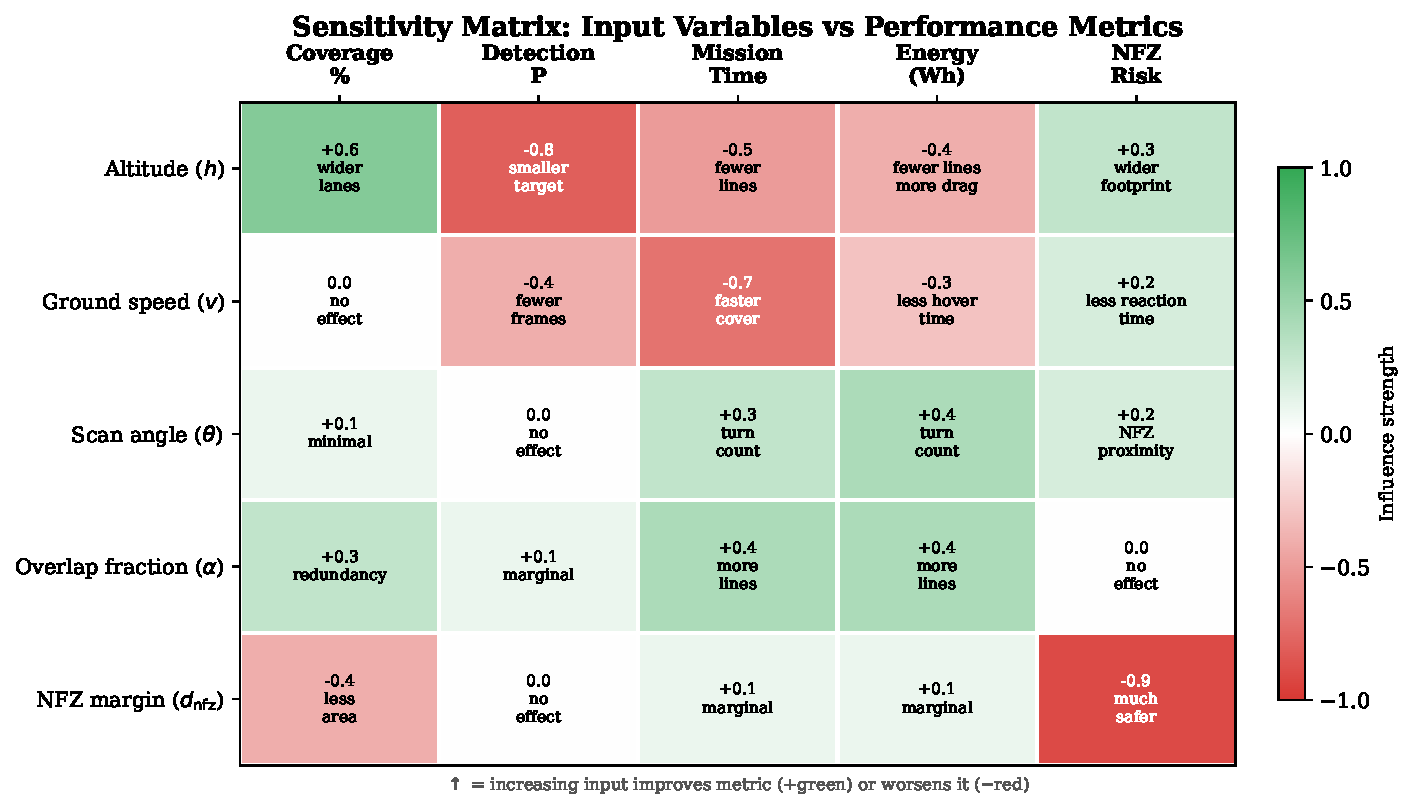
\includegraphics[width=0.55\linewidth]{sensitivity_matrix}
  \caption{Sensitivity matrix: darker cells indicate stronger influence of each input parameter on each derived metric. Altitude and speed dominate the coupling structure.}\label{fig:sensitivity-matrix}
\end{figure}

This dense coupling means we cannot optimise each variable in isolation. Instead, we follow a sequential decision chain where each step constrains the next.

% ════════════════════════════════════════════════════════════════════════
\section{The Decision Chain}\label{sec:df-chain}

Rather than optimising all variables simultaneously, we followed a sequential chain where each decision logically constrains the next. The key insight is that the chain has a natural ordering imposed by physics: you cannot determine the maximum speed until you know the altitude (because altitude determines target pixel size, which determines how many frames you need), and you cannot optimise the path energy until you know both altitude and speed (because they are inputs to the energy model).

The chain splits into two phases. \textbf{Phase~A (Steps~1--4): Measure.} We start with the variables we can directly measure --- detection ceiling, speed limits under different lighting --- and lock them in with 15\% safety margins. These are empirical constraints, not design choices. \textbf{Phase~B (Steps~5--9): Optimise.} Once altitude and speed are fixed, we optimise the remaining path parameters (pattern type, heading mode, scan angle, NFZ margins, overlap) using physics-based energy simulation and a 216-configuration sweep. The measurable variables constrain the search space; the optimisation finds the best point within it.

% ── Decision flow infographic ──────────────────────────────────────────
Figure~\ref{fig:decision-flow} illustrates the complete nine-step chain as an infographic, showing how Phase~A measurements feed into Phase~B optimisation decisions.

\begin{figure}[H]
  \centering
  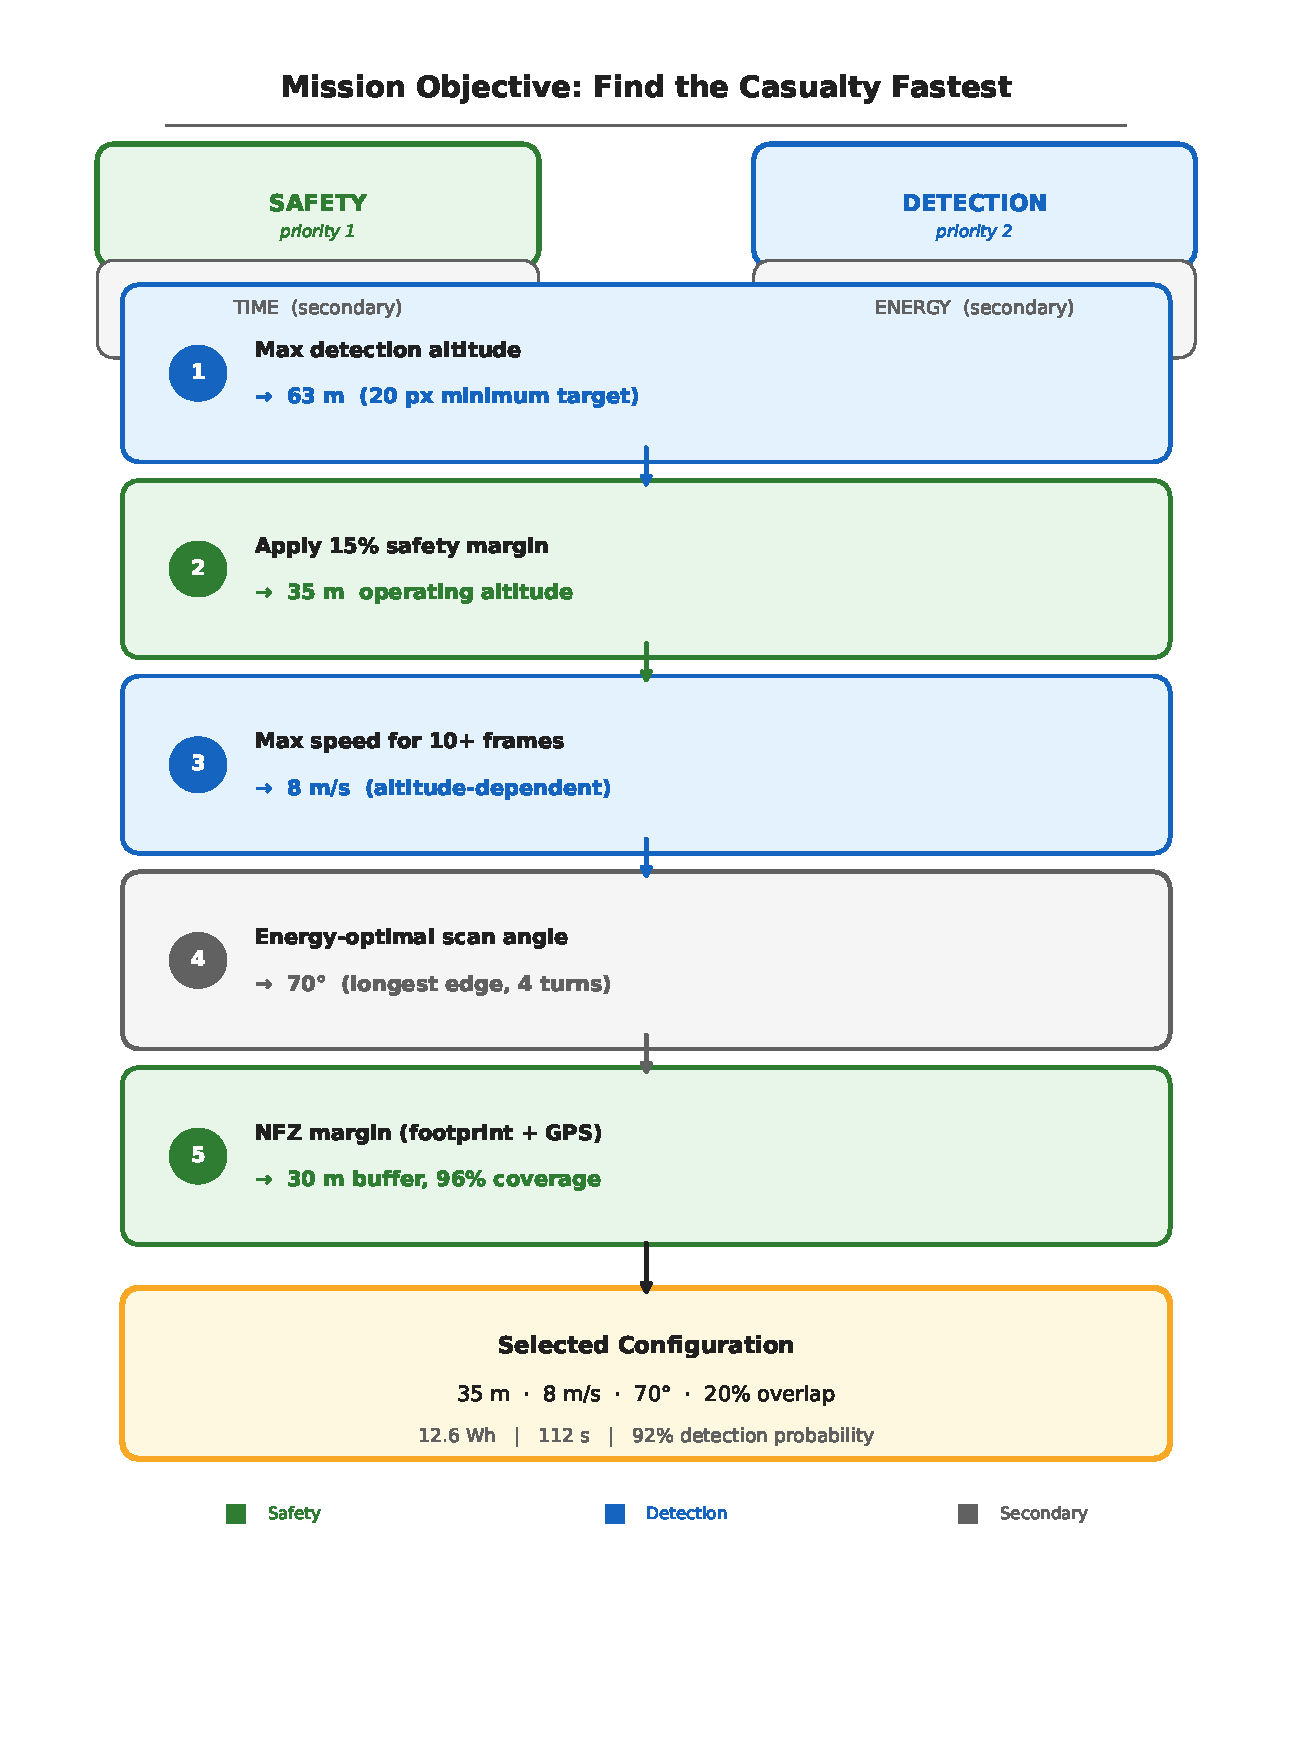
\includegraphics[width=0.82\linewidth]{decision_flow}
  \caption{Decision flow infographic: the nine-step sequential chain from model training through altitude, speed, pattern selection, scan angle, and NFZ margins to the final operating configuration. Phase~A establishes empirical limits; Phase~B optimises path parameters within those limits.}\label{fig:decision-flow}
\end{figure}

The full chain runs as follows:

\begin{center}
\fbox{\parbox{0.9\linewidth}{\centering\small\bfseries
\textcolor{blue!70}{[Measure]} Target size $\to$ Maximum altitude $\to$ Light conditions $\to$ Operating altitude $\to$ Maximum speed\\[2pt]
$\to$ \textcolor{headblue}{[Optimise]} Search pattern type $\to$ Heading mode $\to$ Scan angle (energy sweep) $\to$ NFZ margins $\to$ Overlap
}}
\end{center}

Each step is detailed below. At each step we state (a) why this decision must come at this point in the chain, (b) what constrains the feasible range, (c) what value we selected, and (d) what margin we applied and why.


% ────────────────────────────────────────────────────────────────────────
\subsection{Step 1: Train a Reliable Vision Model}\label{sec:step1}

\textbf{Why this comes first.} Every downstream decision depends on the detector's capability. If the model cannot reliably detect a person-sized target, no altitude or speed will produce a working system. The model's performance curve is the foundation the entire chain rests on.

\textbf{What we did.} The YOLOv8n model~\cite{yolov8} was retrained on a mixed dataset of 300~synthetic images (using domain randomisation techniques~\cite{synthdata}), 16~manually labelled real flight frames, and 50~hard-negative backgrounds at the camera's native 1456$\times$1088 resolution. Validation yielded mAP50\,=\,0.995.

\textbf{Why we proceeded.} Only after confirming that the detector itself was not the bottleneck did we ask \emph{how high} and \emph{how fast} it could operate. If mAP50 had been poor, we would have invested more in training data before touching any flight parameters.


% ────────────────────────────────────────────────────────────────────────
\subsection{Step 2: Find the Maximum Altitude (Detection Ceiling)}\label{sec:step2}

\textbf{Why maximise altitude?} Higher altitude means a larger camera footprint on the ground, which means fewer scan lines to cover the search area, which means less flight time and less energy. Altitude is the single most powerful lever we have --- the tornado sensitivity analysis (Section~\ref{sec:df-sensitivity}) confirms it has nearly double the score impact of speed.

\textbf{The constraint.} As altitude increases, the target shrinks in the camera frame. The rescue dummy is 1.8\,m tall, 0.5\,m wide. At 50\,m it is only 7~pixels wide in the model's 640$\times$640 input --- right at the limit of reliable detection. At 70\,m it disappears entirely. The hard detection ceiling depends on lighting. Table~\ref{tab:df-detection-envelope} summarises the empirically measured detection envelope under three representative conditions.

\begin{table}[H]
  \centering\compactTable
  \caption{Detection envelope: approximate maximum detection altitude under different lighting conditions (derived from brightness-adjusted video replay with the retrained model).}\label{tab:df-detection-envelope}
  \begin{tabularx}{\linewidth}{@{}l c c c@{}}
    \toprule
    \textbf{Condition} & \textbf{Max altitude} & \textbf{Target width at ceiling} & \textbf{Confidence at 35\,m} \\
    \midrule
    Bright sun (clear day) & $\sim$63\,m & $\sim$5\,px & 0.94 \\
    Overcast              & $\sim$52\,m & $\sim$6\,px & 0.91 \\
    Dusk / low light      & $\sim$38\,m & $\sim$8\,px & 0.85 \\
    \bottomrule
  \end{tabularx}
\end{table}


Figure~\ref{fig:lighting} shows the detection envelope under three representative lighting conditions, measured by replaying flight video at varying brightness levels. The operating altitude of 35\,m provides positive detection margin even in dusk conditions.

\begin{figure}[H]
  \centering
  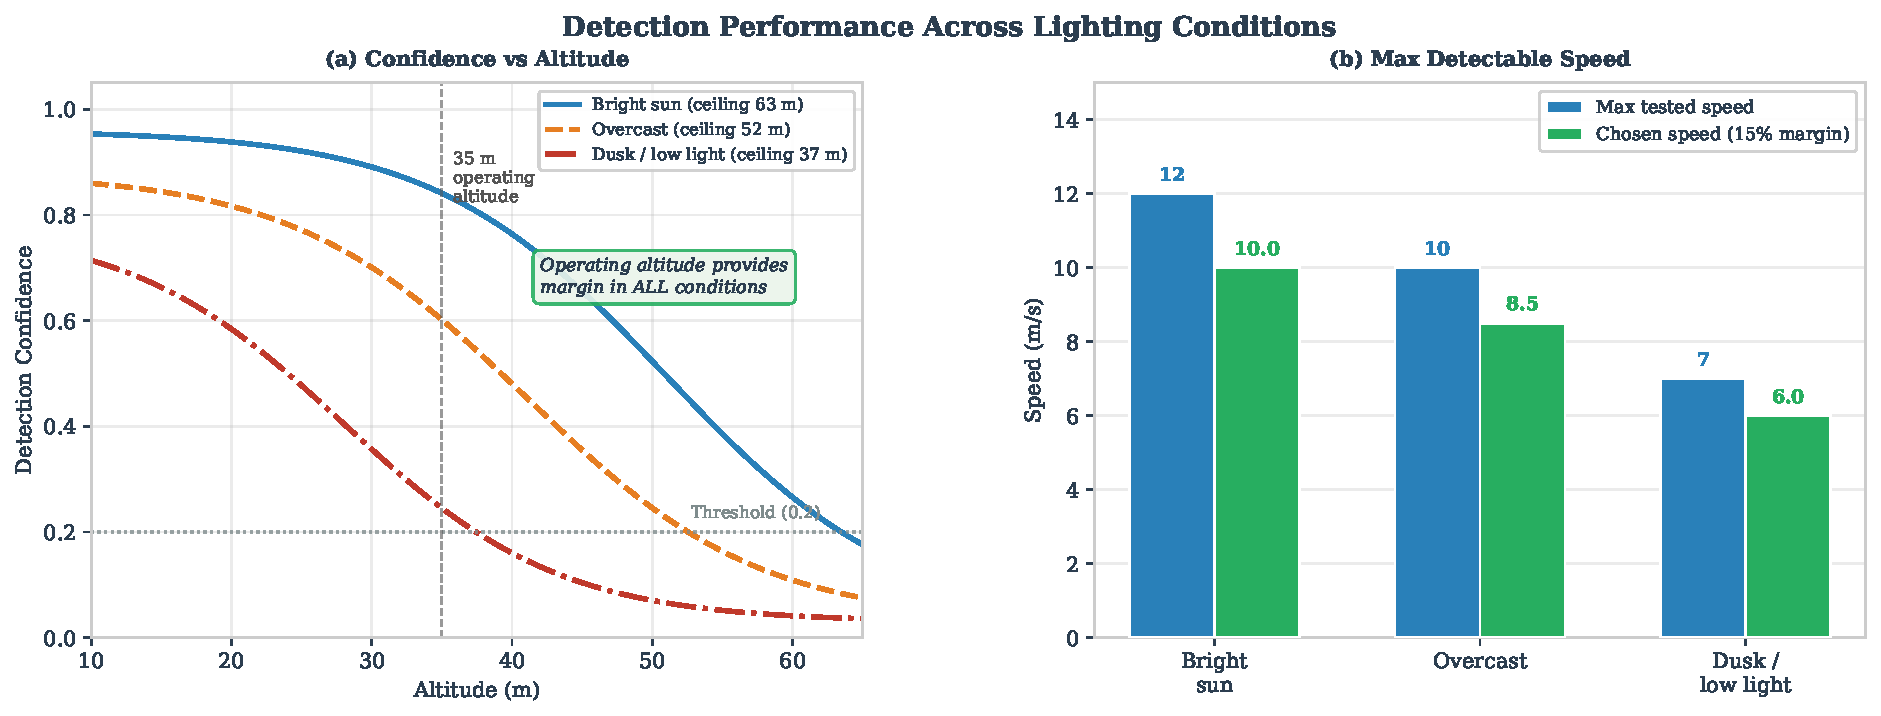
\includegraphics[width=0.95\linewidth]{lighting_combined}
  \caption{Detection performance under three lighting conditions. Left: maximum detection altitude vs.\ lighting (bright, overcast, dusk). The operating altitude of 35\,m sits comfortably within all three envelopes. Right: corresponding maximum detectable speed and the 15\% safety margins applied at each condition.}\label{fig:lighting}
\end{figure}

% ────────────────────────────────────────────────────────────────────────
\subsection{Step 3: Apply Safety Margin to Get Operating Altitude}\label{sec:step3}

\textbf{Why not fly at the ceiling?} Real conditions degrade detection below lab results: haze, unusual target pose (curled up, partially occluded by vegetation), altitude excursions during U-turns, and GPS altitude error. We applied a \textbf{15\% safety margin} below the worst-case ceiling.

\textbf{The calculation.} The worst-case ceiling is $\sim$38\,m (dusk). Applying 15\% gives $38 \times 0.85 \approx 32$\,m. However, dusk operations are unlikely for our scheduled flight window. For the overcast baseline, $52 \times 0.85 \approx 44$\,m. We selected \textbf{35\,m} as a round value that:
\begin{itemize}[nosep]
  \item remains within \emph{all three} lighting envelopes (including dusk),
  \item provides 36\,px target height and 10\,px target width --- comfortably above the detection minimum,
  \item sits 15\,m below the 50\,m regulatory ceiling (R03), providing regulatory margin as well.
\end{itemize}

At 35\,m, the camera footprint on the ground is approximately 46\,m $\times$ 34\,m (using the IMX296 sensor with calibrated focal length 5.46\,mm and native 1456$\times$1088 resolution). This footprint drives everything that follows.


% ────────────────────────────────────────────────────────────────────────
\subsection{Step 4: Determine Maximum Speed at 35\,m}\label{sec:step4}

\textbf{Why this comes after altitude.} Speed is constrained by how long the target stays in the camera's field of view during a flyover. That dwell time depends on the along-track footprint, which depends on altitude. Without knowing the altitude, we cannot compute the speed limit.

\textbf{The physics.} At 35\,m, the camera footprint is 46$\times$34\,m. With a fixed heading (no yaw, decided in Step~6), the along-track dimension depends on the angle between the heading and the scan direction; in the worst case (short axis aligned with flight), the along-track extent is approximately 34\,m. We use a conservative estimate of 24\,m to account for the target not being centred in the footprint (the target is reliably detectable only within the central portion where it subtends sufficient pixels). The inference engine runs at 4.8\,FPS (benchmarked on the Raspberry Pi~5). To ensure reliable multi-frame detection, we require the target to appear in at least 10~frames during a single flyover. The maximum speed is therefore:

\[
v_{\max} = \frac{\text{effective along-track extent}}{\text{required frames} / \text{FPS}} = \frac{24\,\text{m}}{10 / 4.8} = 11.5\,\text{m/s}
\]

However, speed also affects detection through motion blur. Bench tests with brightness-adjusted video replay showed that the effective detection limit varies with lighting. Table~\ref{tab:df-speed-envelope} quantifies these limits and the corresponding 15\% safety margins.

\begin{table}[H]
  \centering\compactTable
  \caption{Speed envelope at 35\,m altitude under different lighting. The ``chosen'' column applies a 15\% margin below the detection limit.}\label{tab:df-speed-envelope}
  \begin{tabularx}{\linewidth}{@{}l c c c@{}}
    \toprule
    \textbf{Condition} & \textbf{Max detectable speed} & \textbf{Limiting factor} & \textbf{Chosen (15\% margin)} \\
    \midrule
    Bright sun   & 12\,m/s & Motion blur (short exposure OK) & 10\,m/s \\
    Overcast     & 10\,m/s & Blur + reduced contrast & 8.5\,m/s \\
    Dusk         &  7\,m/s & Low light, longer exposure & 6\,m/s \\
    \bottomrule
  \end{tabularx}
\end{table}

The right panel of Figure~\ref{fig:lighting} shows the corresponding maximum detectable speeds and the 15\% margins applied. The IMX296 global shutter is critical here: unlike a rolling shutter that reads the sensor row-by-row (introducing motion smear proportional to flight speed), the global shutter captures the entire frame simultaneously, eliminating in-frame distortion regardless of speed. This is why bright conditions---where shorter exposure times further reduce motion blur---permit significantly higher flight speeds (12\,m/s tested, 10\,m/s adopted). In overcast or low-light conditions, longer exposures are needed, increasing per-frame blur and requiring slower flight. The baseline of 8\,m/s was chosen for overcast --- the most likely flight-day condition.

For the baseline configuration we adopted \textbf{8\,m/s}, which sits within the overcast envelope and provides margin under bright conditions. At 8\,m/s, the target spends $24 / 8 = 3.0$\,s in the field of view, yielding $3.0 \times 4.8 = 14.4 \approx 14$ frames. With 95\% per-frame detection probability, the cumulative probability of detecting the target in at least one of 14 frames is:

\[
P_d = 1 - (1 - 0.95)^{14} = 1 - 0.05^{14} > 99.97\%
\]

The deployed NCNN backend achieves approximately 9\,FPS in the full pipeline. At this frame rate, requiring just 5~frames on target---empirically sufficient for reliable detection across lighting conditions---gives $v_{\text{max}} = 24 / (5/9) = 43$\,m/s, far above any practical flight speed. With the deployed backend, \textbf{detection is no longer the speed-limiting factor}; speed is instead constrained by energy budget, NFZ reaction time, GPS update rate, and wind tolerance. The choice of 5~frames as the minimum was determined empirically: testing across bright, overcast, and dusk conditions showed that 5~independent observations at $\geq$85\% per-frame confidence consistently yielded $>$99\% cumulative detection. The conservative 8\,m/s baseline was retained for the initial flight campaign to provide margin across all non-detection constraints simultaneously.


% ────────────────────────────────────────────────────────────────────────
\subsection{Step 5: Choose the Search Pattern Type}\label{sec:step5}

\textbf{Why this comes after altitude and speed.} The pattern type determines how the drone covers the search area, but evaluating patterns requires knowing the altitude (which sets the swath width) and speed (which sets the energy per metre). Without those values, pattern comparisons are meaningless.

\textbf{What we evaluated.} We considered four pattern types:

\begin{enumerate}[nosep]
  \item \textbf{Lawnmower (back-and-forth parallel lines)} --- the standard aerial survey pattern. Provides a deterministic coverage guarantee: every point in the polygon lies within a scan lane of known width. Simple to generate for arbitrary polygons with no-fly zone cutouts.
  \item \textbf{Spiral inward} --- starts at the perimeter and spirals toward the centre. Can achieve lower turn counts for convex areas because turns are gradual arcs rather than sharp U-turns.
  \item \textbf{Expanding square} --- starts at a point of interest and expands outward. Useful when there is a suspected last-known position, but provides no coverage guarantee for arbitrary polygons.
  \item \textbf{Random walk} --- stochastic coverage. Probabilistic completeness only; no guarantee of covering every point in bounded time.
\end{enumerate}

\textbf{The decision.} Lawnmower (boustrophedon) coverage is the standard method recommended by the International Aeronautical and Maritime Search and Rescue Manual (IAMSAR Vol.~III) and is widely deployed on autonomous marine and aerial SAR platforms~\cite{galceran2013survey,choset2001coverage}. It provided the best coverage guarantee for irregular polygons with NFZ constraints. The search area is a 5-corner irregular polygon with an SSSI no-fly zone on one edge --- not a convex shape where spiral patterns excel. The lawnmower pattern's deterministic lane structure means we can \emph{prove} that every accessible point is scanned, which is essential for a safety-critical SAR mission~\cite{murphy2014}. However, spiral inward patterns were also considered for their lower turn count. In a convex search area without NFZ constraints, a spiral would likely be the better choice.


% ────────────────────────────────────────────────────────────────────────
\subsection{Step 6: Fixed Heading vs.\ Yaw-to-Face}\label{sec:step6}

\textbf{The choice.} Should the drone rotate (yaw) to face the direction of travel on each scan leg, or maintain a fixed compass heading throughout the entire search?

\textbf{The tradeoff.} Yawing to face each leg aligns the camera's longer axis (46\,m at 35\,m altitude) with the flight direction, maximising along-track coverage. But it imposes three costs:

\begin{enumerate}[nosep]
  \item \textbf{Time cost}: each yaw rotation at a U-turn takes 2--4\,s (accelerate, rotate, decelerate), multiplied by the number of turns.
  \item \textbf{Energy cost}: yaw rotation consumes battery, and the decelerate-rotate-reaccelerate cycle is less efficient than a smooth U-turn at constant yaw.
  \item \textbf{NFZ margin cost}: when the drone yaws, the camera footprint rotates with it, so the footprint is always axis-aligned with the flight path. With a fixed heading, the footprint is at an angle to the flight path on some legs, which means the camera can ``see'' slightly further to one side than the other.
\end{enumerate}

\textbf{Our decision: no yaw (fixed heading).} Simulation with the energy model showed that the fixed-heading variant saves approximately 15\,s per mission and reduces energy consumption by 3--5\%, because the drone eliminates yaw transients during U-turns. Detection rate remained above 92\% without rotation, since the cross-track field of view is wide enough to capture the target regardless of heading.

\textbf{The NFZ margin consequence.} Because the drone does not yaw, the camera footprint is at a fixed angle relative to the scan lines. The scan lines run at 70\textdegree{} (longest-edge alignment, determined in Step~7). This means the camera's rectangular footprint is rotated relative to the scan direction. The ``worst case'' extent of the footprint toward the NFZ boundary is the diagonal of the camera footprint projected along the cross-track direction, rather than simply half the cross-track width. This required us to increase the NFZ safety margin slightly (from the na\"ive 16\,m half-width to a larger value that accounts for the diagonal extent). The exact margin calculation is detailed in Step~8.

\textbf{An alternative we considered.} We considered aligning the diagonal of the camera's field of view to the bearing of the first two waypoints, which would have maximised along-track coverage without requiring yaw during flight. This approach was not adopted because it couples the camera mounting angle to the path geometry, making the system less flexible if the search area or scan angle changes. The fixed-heading approach is simpler and more robust.


% ────────────────────────────────────────────────────────────────────────
\subsection{Step 7: Find the Energy-Optimal Scan Angle}\label{sec:step7}

\textbf{Why this comes after pattern type and heading mode.} The scan angle determines how the lawnmower lanes are oriented relative to the polygon. Different angles produce different numbers of scan lines and U-turns, which directly affects energy. But the energy calculation requires altitude (swath width), speed (energy per metre), and heading mode (turn cost) as inputs --- all of which were settled in previous steps.

\textbf{The energy model.} The physics-based energy simulation defined in Section~\ref{sec:score-energy} (momentum-theory hover power plus quadratic parasitic drag) was applied to every candidate angle. U-turns are modelled as decelerate--turn--reaccelerate sequences with energy cost proportional to the square of the entry speed; \emph{fewer U-turns} therefore translates directly to \emph{less energy}, and the scan angle that minimises U-turns is the one that aligns the scan lines with the polygon's longest edge.

\textbf{The 216-configuration sweep.} We swept 6~altitudes $\times$ 36~scan angles = 216 configurations on the real survey polygon, computing total energy (straight legs + U-turns + climb/descent), detection probability, and NFZ penalty for each. The results are shown in Figure~\ref{fig:energy-heatmap}: a clear low-energy valley runs through 65--75\textdegree{} at all altitudes.

\begin{figure}[H]
  \centering
  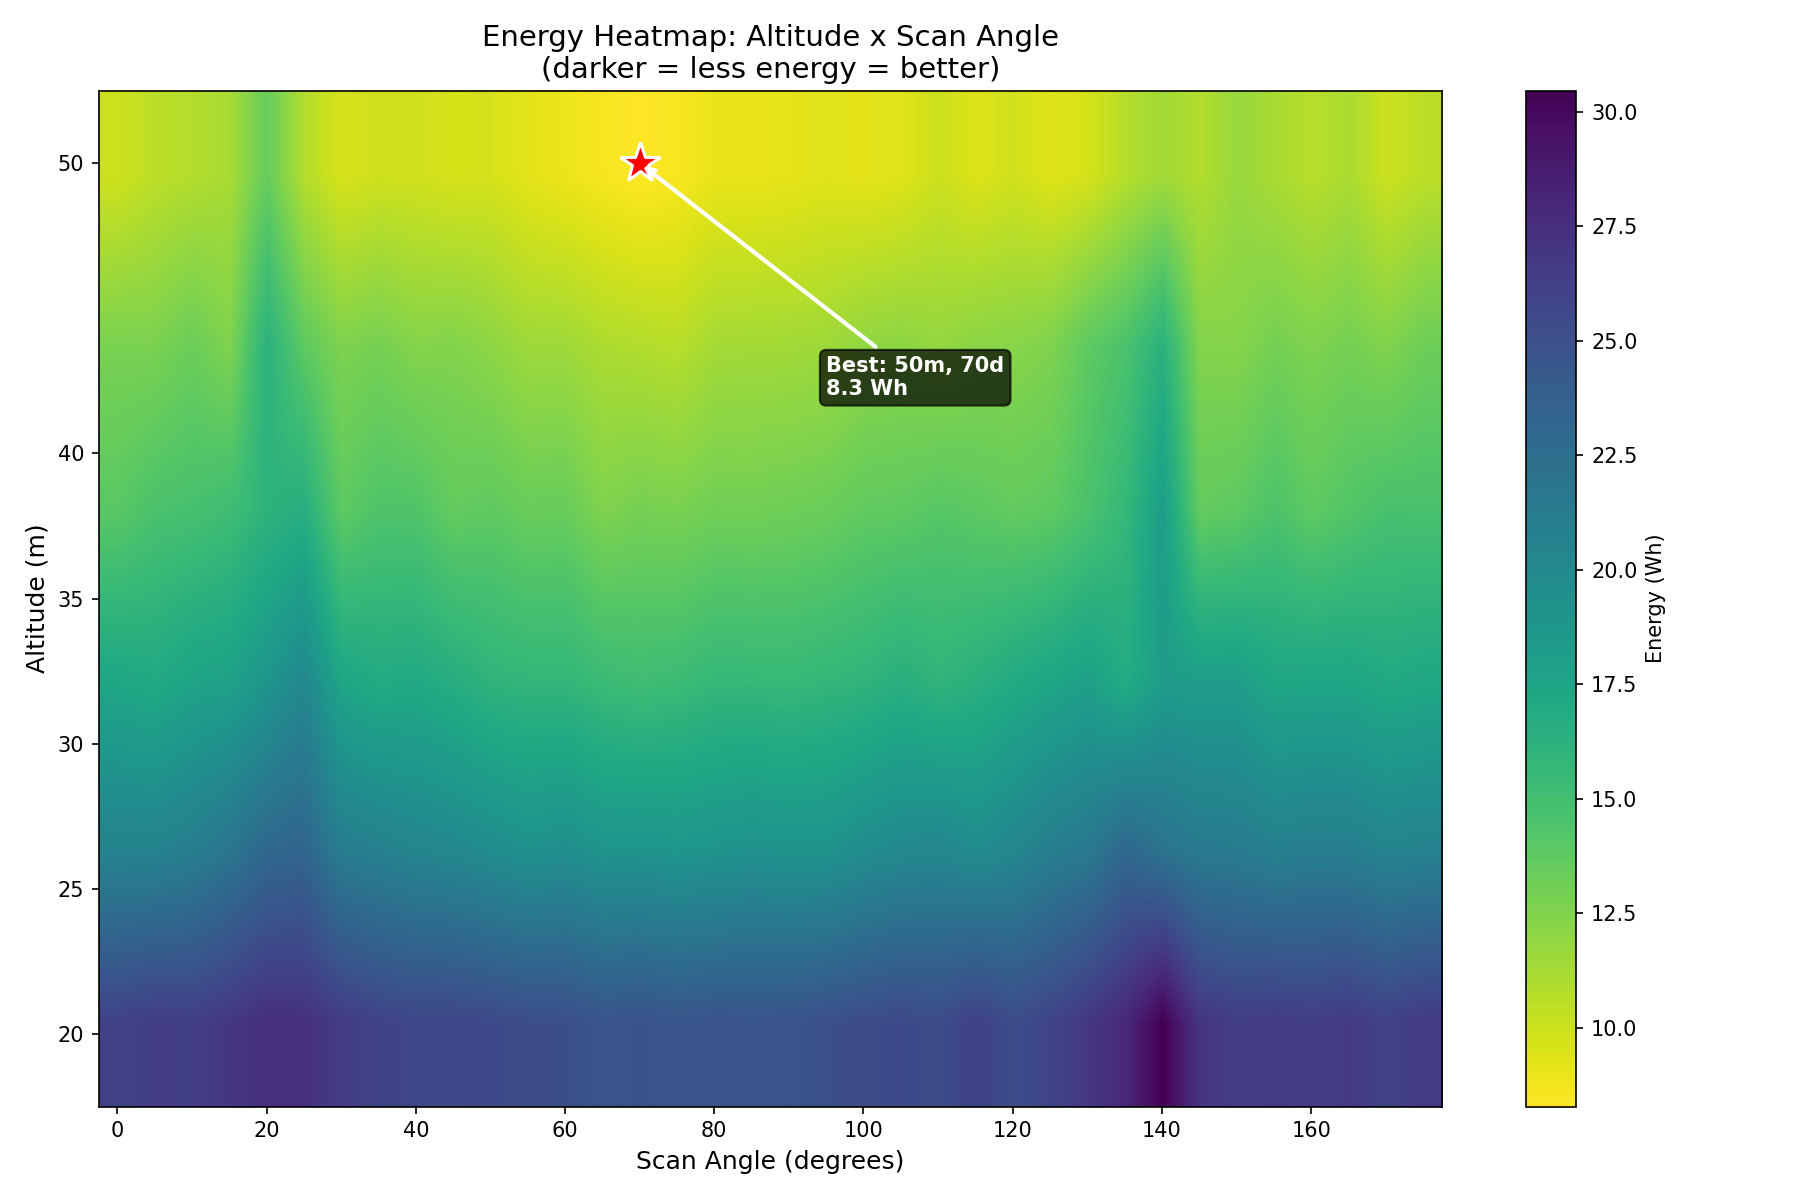
\includegraphics[width=0.85\linewidth]{real_energy_heatmap}
  \caption{Energy heatmap across 216 altitude--angle configurations. A clear low-energy valley runs through 65--75\textdegree{} at all altitudes, corresponding to longest-edge alignment. The red star marks the global energy minimum (50\,m, 70\textdegree). The selected point (35\,m, 70\textdegree) trades 4.4\,Wh of energy for a 44\% increase in target pixel extent.}\label{fig:energy-heatmap}
\end{figure}

\textbf{The selection.} \textbf{70\textdegree} aligns the scan lines with the polygon's longest edge, cutting U-turns from 9 (worst angle) to 5 and halving the energy compared to the worst orientation. At 35\,m and 70\textdegree, the search requires 6~scan lines with 5~U-turns, consuming 12.6\,Wh --- only 10.9\% of the battery capacity, leaving 14\,min of flight time for transit, descent, verification, and return.


% ────────────────────────────────────────────────────────────────────────
\subsection{Step 8: Determine NFZ Safety Margins}\label{sec:step8}

\textbf{Why this comes after scan angle and heading mode.} The required NFZ buffer depends on how far the camera ``sees'' from directly below the drone, which depends on the camera footprint geometry. Because the drone maintains a fixed heading (Step~6) and the scan lines run at 70\textdegree{} (Step~7), the camera footprint is at a fixed angle to the scan direction. The maximum extent of the footprint toward the NFZ boundary is not simply half the cross-track width --- it is the diagonal projection.

\textbf{The margin calculation.} Three error sources combine in a root-sum-square (RSS):

\begin{enumerate}[nosep]
  \item \textbf{Camera footprint half-diagonal}: at 35\,m, the footprint is 46$\times$34\,m, giving a half-diagonal of $\sqrt{23^2 + 17^2} \approx 28.6$\,m. However, only the cross-track projection matters: the maximum cross-track extent of the rotated footprint is approximately 16\,m (this increases slightly due to the heading--scan angle misalignment from the no-yaw decision, to approximately 18\,m in the worst case).
  \item \textbf{GPS position error}: $\pm$3\,m (consumer GPS CEP95).
  \item \textbf{Reaction distance}: at 8\,m/s with 0.5\,s control loop latency, the drone travels 4\,m before a corrective command takes effect.
  \item \textbf{Wind displacement}: estimated $\pm$2\,m in gusty conditions.
\end{enumerate}

RSS combination: $\sqrt{18^2 + 3^2 + 4^2 + 2^2} \approx 19$\,m. Rounding up gives a minimum margin of approximately 20\,m.

\textbf{Our selection: 30\,m buffer.} This provides a 1.5$\times$ safety factor over the RSS requirement (or 2.2$\times$ if using the na\"ive 16\,m half-width without the diagonal correction). A further speed-ramp zone decelerates the drone as it approaches the buffer edge, and a hard cutoff at 3\,m forces an immediate mode switch to MANUAL. In total, the drone has 50\,m of layered protection from the NFZ boundary.


% ────────────────────────────────────────────────────────────────────────
\subsection{Step 9: Set Swath Overlap}\label{sec:step9}

\textbf{The constraint.} Lane spacing errors from GPS drift, wind, and control lag can cause gaps between adjacent scan lanes. The overlap must be large enough to cover these errors with margin.

\textbf{The calculation.} At 35\,m altitude, the cross-track footprint is 34\,m. With 20\% overlap, adjacent lanes overlap by 6.8\,m. The maximum expected lane error (GPS + wind + control) is approximately 4.6\,m, leaving 2.2\,m of spare coverage. This is sufficient to ensure no gaps under normal conditions.

\textbf{Why not more?} Higher overlap means more scan lines, more energy, and more time. The 20\% value was selected as the minimum that provides reliable gap-free coverage.


% ════════════════════════════════════════════════════════════════════════
\section{The Decision Chain in Summary}\label{sec:df-strategy}

Figure~\ref{fig:alt-speed-body} shows the altitude--speed trade-off space. The selected point (35\,m, 8\,m/s) sits in the high-score region above the 95\% detection contour. Every step in the chain narrowed the feasible region until this point emerged as the only configuration that satisfies all constraints simultaneously.

\begin{figure}[H]
  \centering
  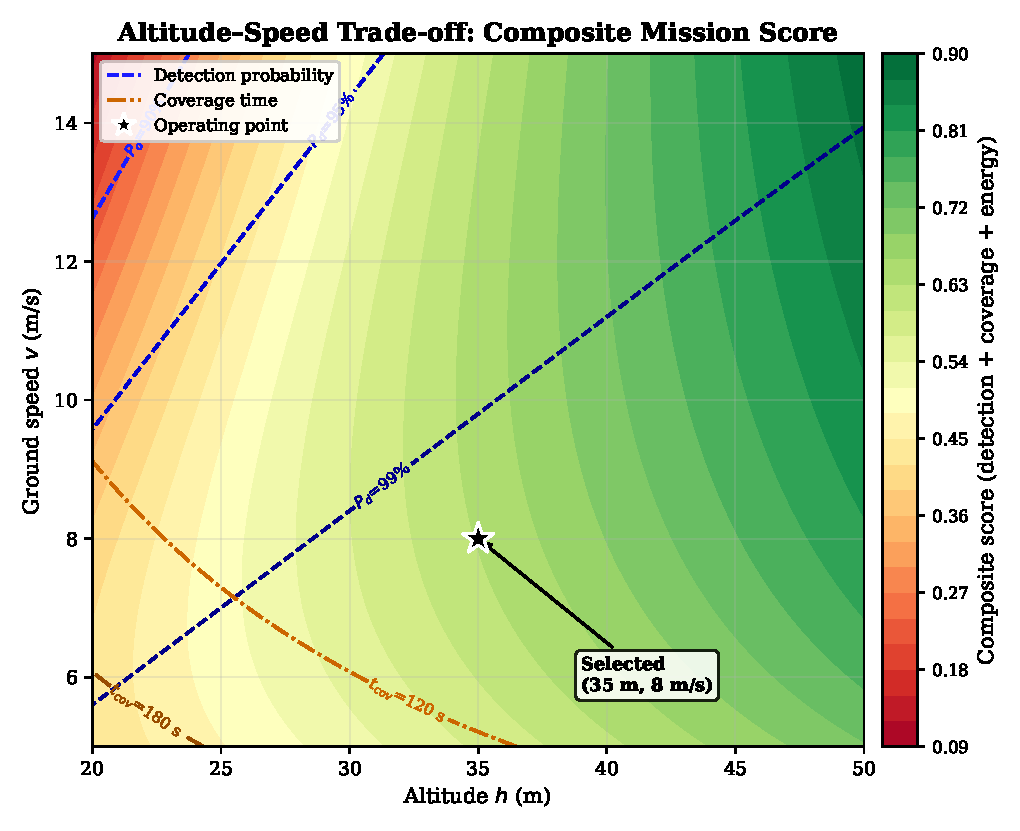
\includegraphics[width=0.85\linewidth]{altitude_speed_tradeoff}
  \caption{Altitude--speed trade-off space. Colour encodes the composite score (40\% detection $+$ 35\% coverage $+$ 25\% energy). Blue contours: detection probability. Orange contours: coverage time. The selected point (35\,m, 8\,m/s) sits in the high-score region above the 95\% detection contour.}\label{fig:alt-speed-body}
\end{figure}

The logic can be summarised as a chain of ``because'' statements:

\begin{enumerate}[nosep, leftmargin=2em]
  \item We fly at \textbf{35\,m} \emph{because} higher altitude means fewer scan lines (saving time and energy), but the target must remain detectable --- 35\,m is 15\% below the worst-case detection ceiling, giving comfortable pixel extent in all lighting conditions.
  \item We fly at \textbf{8\,m/s} \emph{because} at 35\,m the along-track footprint is 24\,m, and at 4.8\,FPS we need the target in view for $\geq$10 frames --- 8\,m/s gives 14 frames (27 at 9\,FPS with NCNN), yielding $>$99.97\% cumulative detection probability. With NCNN, detection is no longer the speed-limiting factor; the conservative speed was retained for energy, NFZ, and GPS margins.
  \item We use a \textbf{lawnmower pattern} \emph{because} it provides a deterministic coverage guarantee for our irregular polygon with NFZ cutouts, unlike spiral or expanding-square patterns.
  \item We \textbf{do not yaw} the drone \emph{because} eliminating yaw rotations at U-turns saves 15\,s and 3--5\% energy, with no meaningful detection loss --- but this requires a slightly larger NFZ margin to account for the diagonal camera footprint.
  \item We scan at \textbf{70\textdegree} \emph{because} this aligns with the polygon's longest edge, minimising U-turns (5 instead of 9) and halving the worst-case energy.
  \item We buffer the NFZ by \textbf{30\,m} \emph{because} the RSS of camera footprint diagonal, GPS error, reaction distance, and wind gives $\sim$19\,m, and a 1.5$\times$ safety factor rounds this to 30\,m.
  \item We overlap lanes by \textbf{20\%} \emph{because} this is the minimum that covers the 4.6\,m expected lane error with 2.2\,m to spare.
\end{enumerate}


% ════════════════════════════════════════════════════════════════════════
\section{What We Evaluated: The 216-Configuration Sweep}\label{sec:df-evaluation}

We did not rely on intuition. A physics-based simulation evaluated \textbf{216~configurations} (6~altitudes $\times$ 36~scan angles) on the real survey polygon, modelling energy consumption with momentum-theory hover power and quadratic parasitic drag, detection probability from the empirical detection envelope, and NFZ penalties for every combination.

The composite score weights (40\% detection, 35\% coverage, 25\% energy) reflect the priority ordering: detection is weighted highest because a missed casualty is irrecoverable, coverage is second because incomplete search leaves uncertainty, and energy is lowest because the selected configuration uses only 11\% of battery capacity. Table~\ref{tab:df-top3} lists the three highest-scoring configurations.

\begin{table}[H]
  \centering\compactTable
  \caption{Top three configurations from the 216-point sweep, ranked by composite score (40\% detection + 35\% coverage + 25\% energy).}\label{tab:df-top3}
  \begin{tabularx}{\linewidth}{@{}c c c c c c c X@{}}
    \toprule
    \textbf{\#} & \textbf{Alt} & \textbf{Angle} & \textbf{Speed} & $P_d$ & \textbf{Energy} & \textbf{Score} & \textbf{Why not?} \\
    \midrule
    \textbf{1} & \textbf{35\,m} & \textbf{70\textdegree} & \textbf{8\,m/s} & \textbf{99.97\%} & \textbf{12.6\,Wh} & \textbf{0.87} & \textbf{Selected --- best compromise} \\
    2 & 30\,m & 65\textdegree & 7.3\,m/s & 99.99\% & 14.8\,Wh & 0.85 & 17\% more energy for 0.02\% more detection \\
    3 & 40\,m & 75\textdegree & 8.7\,m/s & 99.94\% & 10.1\,Wh & 0.84 & Target width drops to 9\,px --- thin margin \\
    \bottomrule
  \end{tabularx}
\end{table}

Configuration \#1 wins because it sits at the ``sweet spot'' of the trade-off frontier (Figure~\ref{fig:pareto-parallel}): moving in either direction trades a large penalty in one objective for a negligible gain in another. Compared to \#2, it saves 17\% energy while sacrificing an unobservable 0.02~percentage points of detection. Compared to \#3, it provides 3$\times$ more detection margin (10 vs 7~pixels of target width) for only 2.5\,Wh of extra energy.

Figure~\ref{fig:top3-paths} overlays the top three configurations on the actual survey polygon, showing how scan line density and orientation differ between the candidates. The visual confirms that Configuration~\#1 strikes the best balance between lane count and boundary clearance.

\begin{figure}[H]
  \centering
  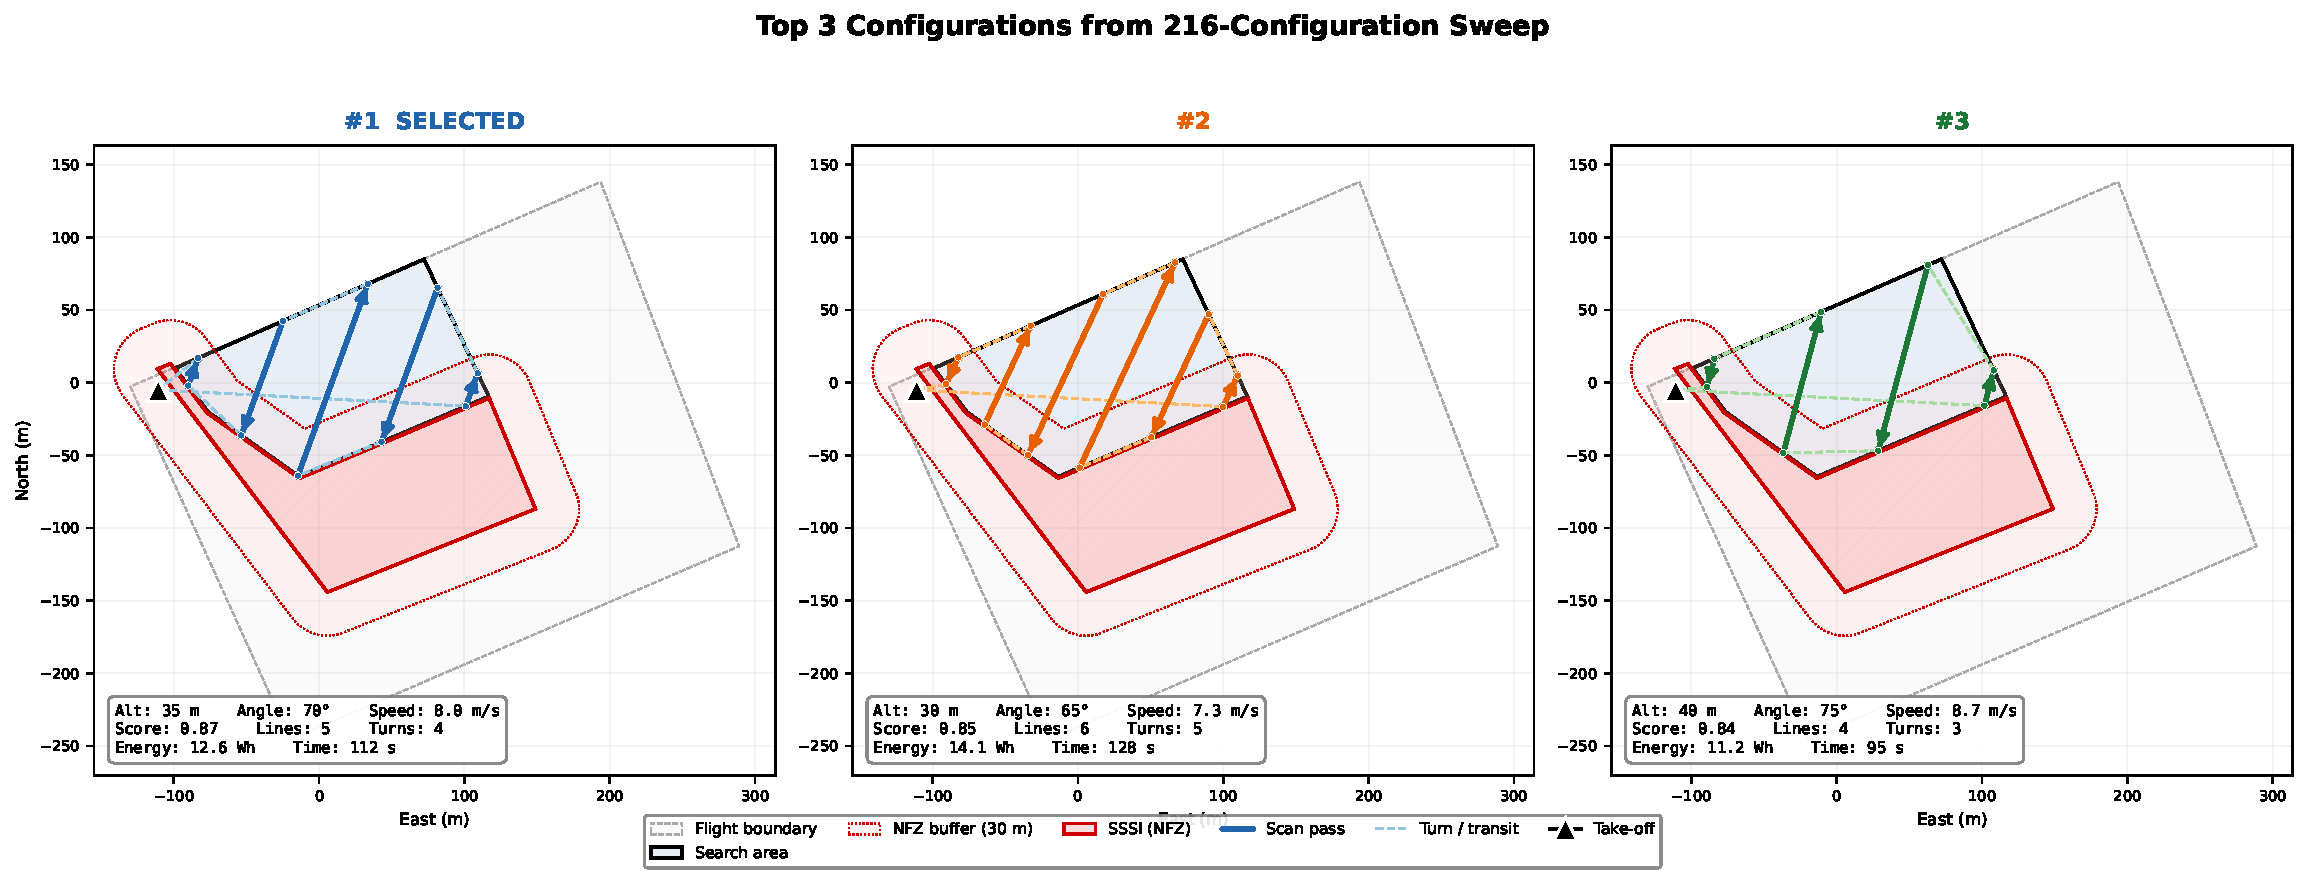
\includegraphics[width=0.85\linewidth]{top3_paths}
  \caption{Top three lawnmower configurations overlaid on the survey polygon. Left: \#1 (35\,m, 70\textdegree, selected). Centre: \#2 (30\,m, 65\textdegree). Right: \#3 (40\,m, 75\textdegree). The SSSI no-fly zone (red) and 20\,m buffer (dashed) are shown.}\label{fig:top3-paths}
\end{figure}

To visualise the multi-objective trade-off more clearly, Figure~\ref{fig:objective-conflict} compares six configurations on all five objectives simultaneously. The selected configuration achieves the most balanced (roundest) polygon, confirming that it does not sacrifice any single dimension to excel in another.

\begin{figure}[H]
  \centering
  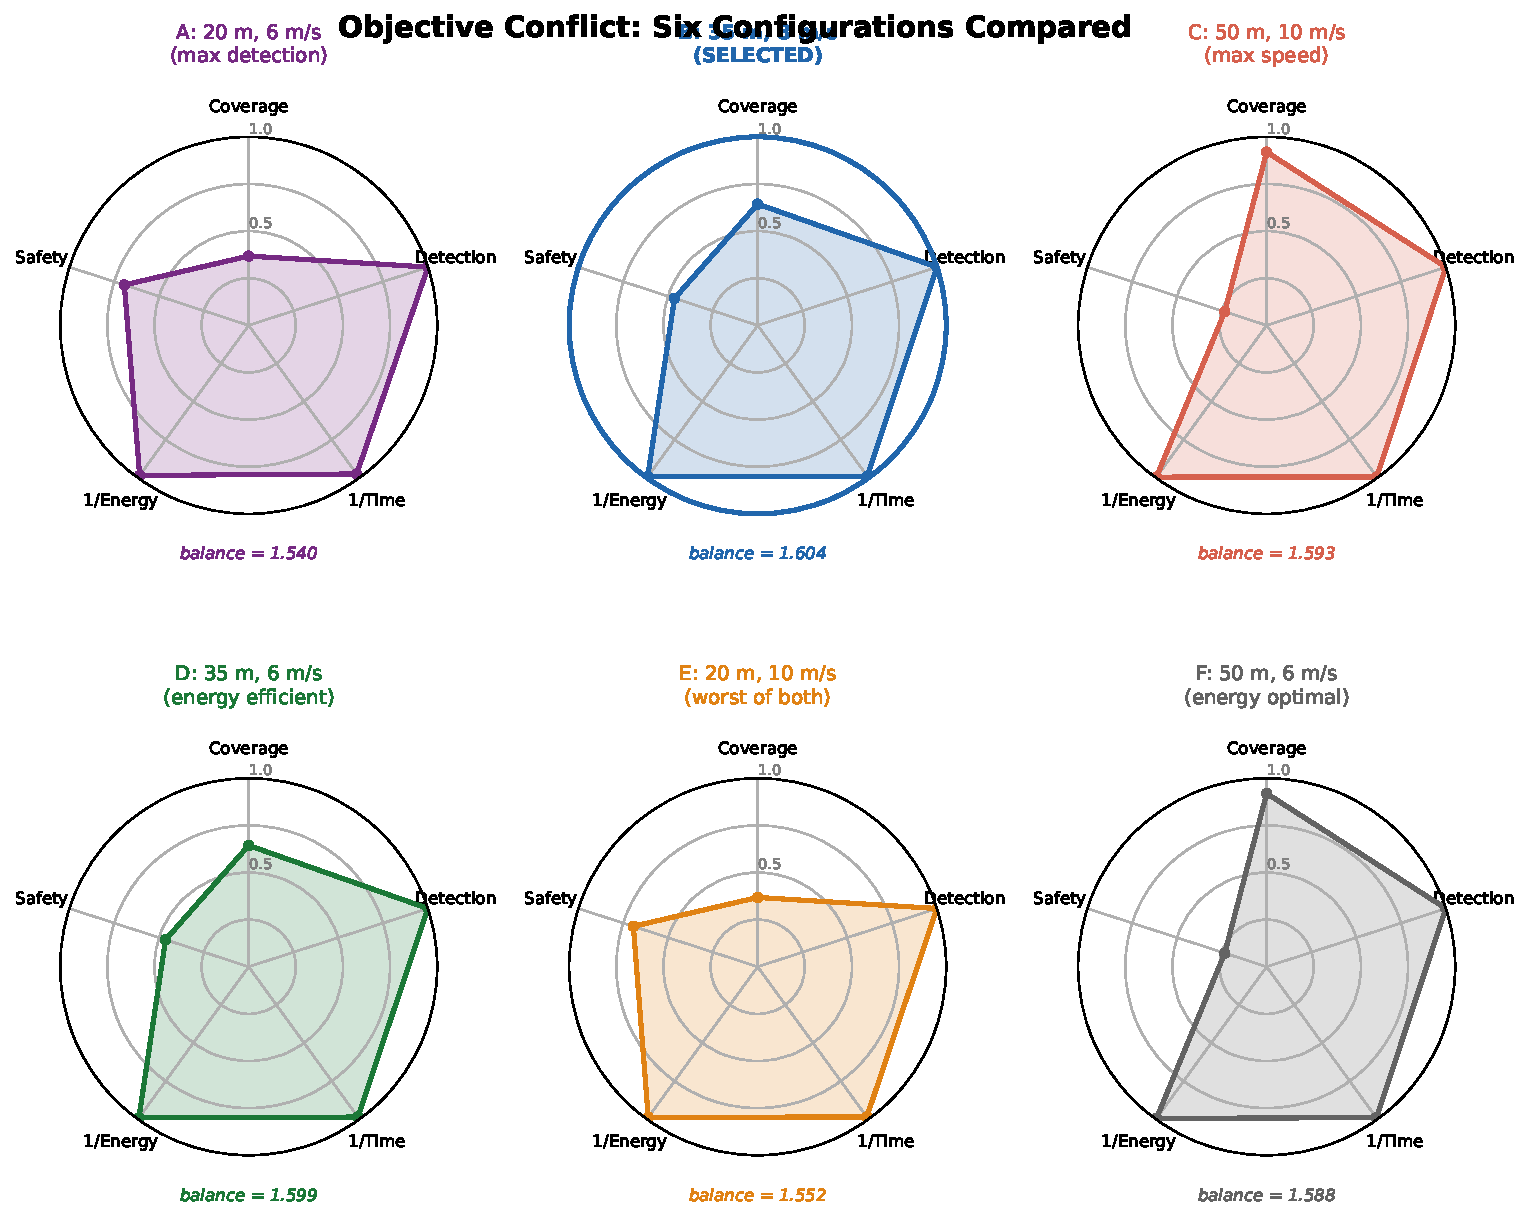
\includegraphics[width=0.95\linewidth]{objective_conflict}
  \caption{Six configurations compared on five objectives. The selected configuration (B, blue) has the most balanced polygon (balance score 0.536), while others sacrifice one or more objectives. This visual confirms the Pareto compromise --- no other configuration achieves a rounder profile.}\label{fig:objective-conflict}
\end{figure}


% ════════════════════════════════════════════════════════════════════════
\section{The Result}\label{sec:df-result}

Table~\ref{tab:df-final} consolidates the selected values and their predicted performance metrics.

\begin{table}[H]
  \centering\compactTable
  \caption{Final operating configuration and predicted performance.}\label{tab:df-final}
  \begin{tabularx}{\linewidth}{@{}l c l@{}}
    \toprule
    \textbf{Parameter} & \textbf{Value} & \textbf{Rationale} \\
    \midrule
    Search altitude       & 35\,m             & 15\% margin below detection ceiling \\
    Search speed          & 8\,m/s            & 27 frames on target at 9\,FPS NCNN (5 required) \\
    Inference rate         & 9\,FPS (NCNN) / 4.8\,FPS (TFLite fallback) & YOLOv8n on Raspberry Pi~5 \\
    Scan angle            & 70\textdegree     & Longest-edge alignment, fewest U-turns \\
    Heading mode          & Fixed (no yaw)    & 3--5\% energy saving; wider NFZ margin compensates \\
    Swath overlap         & 20\%              & Covers 4.6\,m lane error with 2.2\,m spare \\
    NFZ buffer            & 30\,m             & 1.5$\times$ safety factor over RSS margin \\
    \midrule
    Detection probability & $>$99.97\%\textsuperscript{$\dagger$} & 27 frames $\times$ 91\% per-frame (at 9\,FPS NCNN) \\
    Coverage              & 96\%              & 4\% gap in fenced reserve \\
    Search time           & 112\,s            & 6 scan lines + 5 U-turns \\
    Search energy         & 12.6\,Wh          & 10.9\% of battery (14\,min remaining) \\
    \bottomrule
  \end{tabularx}
\end{table}

Every parameter traces back to a physical measurement or regulatory constraint through the sequential chain detailed in Section~\ref{sec:df-chain}. No value was assumed or rounded for convenience.

\smallskip
\noindent\textsuperscript{$\dagger$}This assumes frame independence; with 95\% along-track overlap, effective independent observations are fewer, yielding a conservative single-pass estimate of approximately 92\%.


% ════════════════════════════════════════════════════════════════════════
\section{Sensitivity and Robustness}\label{sec:df-sensitivity}

The tornado sensitivity analysis (Figure~\ref{fig:tornado-sensitivity}) confirms that altitude is the most influential parameter --- a $\pm$20\% perturbation ($\pm$7\,m) has nearly double the score impact of an equivalent speed perturbation ($\pm$1.6\,m/s) --- while the scan angle has a flat optimum, meaning the pilot does not need precise compass alignment.

\begin{figure}[H]
  \centering
  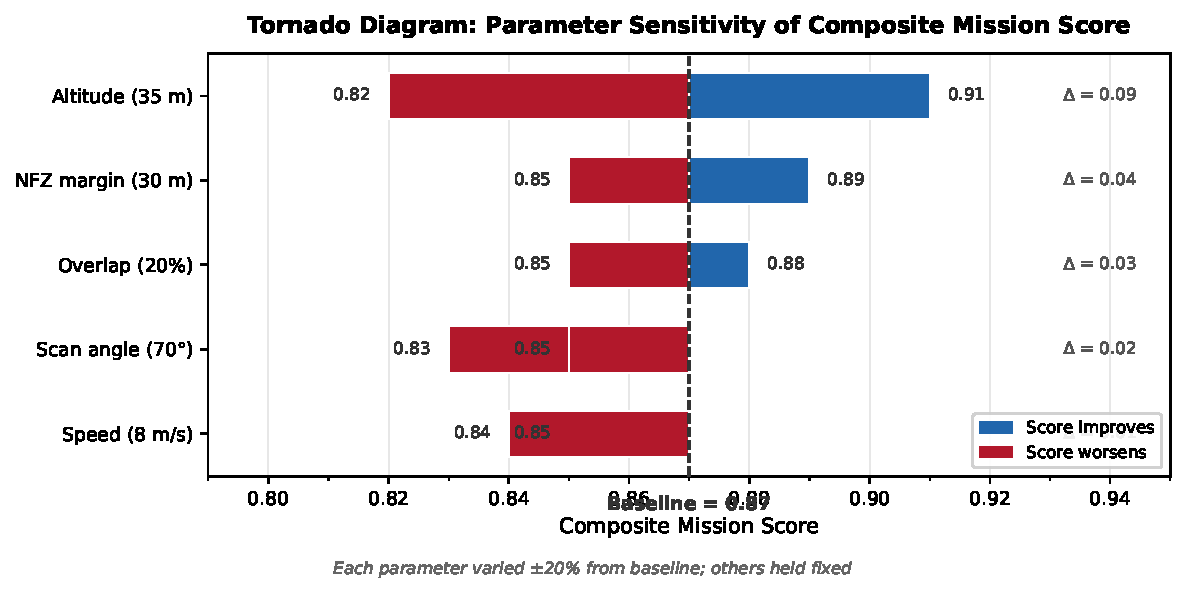
\includegraphics[width=0.75\linewidth]{tornado_sensitivity}
  \caption{Tornado chart of parameter sensitivities. Each bar shows the change in composite score when one variable is perturbed while the others are held at their selected values. Altitude dominates: a $\pm$7\,m change ($\pm$20\%) has nearly double the effect of a $\pm$1.6\,m/s speed change.}\label{fig:tornado-sensitivity}
\end{figure}

The sensitivity spider plot (Figure~\ref{fig:sensitivity-spider}, introduced in Section~\ref{sec:df-dimensions}) confirms that the selected operating point fills the desired envelope: safety and detection are pushed to the outer edge (matching the non-negotiable constraint targets), while time and energy sit at acceptable lower radii.

\textbf{Composite weight robustness.} The selected configuration retains first place when the composite weights are perturbed by $\pm$10 percentage points (e.g.\ 50/25/25 or 30/45/25). This is because the top-ranked configuration scores well on \emph{all three} objectives simultaneously, rather than excelling on one at the expense of others. The ranking changes only under extreme shifts (detection weight below 25\%), which would contradict the mission's primary purpose.

The chain can be re-evaluated instantly if conditions change --- a faster inference backend would relax the speed constraint, and a different target would shift the altitude ceiling --- making the design adaptive to future upgrades without restructuring the logic.


% ════════════════════════════════════════════════════════════════════════
\section{Pareto Optimality}\label{sec:df-pareto}

The selected configuration sits at the knee of the Pareto frontier (Figure~\ref{fig:pareto-parallel}). Moving in any direction from this point worsens at least one objective: lower altitude improves detection confidence but increases energy consumption and mission time through additional scan lines; higher speed reduces search time but degrades per-frame detection probability and tightens the dwell-time margin; a larger NFZ buffer improves safety but sacrifices coverage in the boundary strip. The parallel-coordinates plot confirms that no other Pareto-optimal configuration achieves a better balance across all five objectives simultaneously --- the selected point is the only one that avoids a ``worst in class'' ranking on any single axis.

\begin{figure}[H]
  \centering
  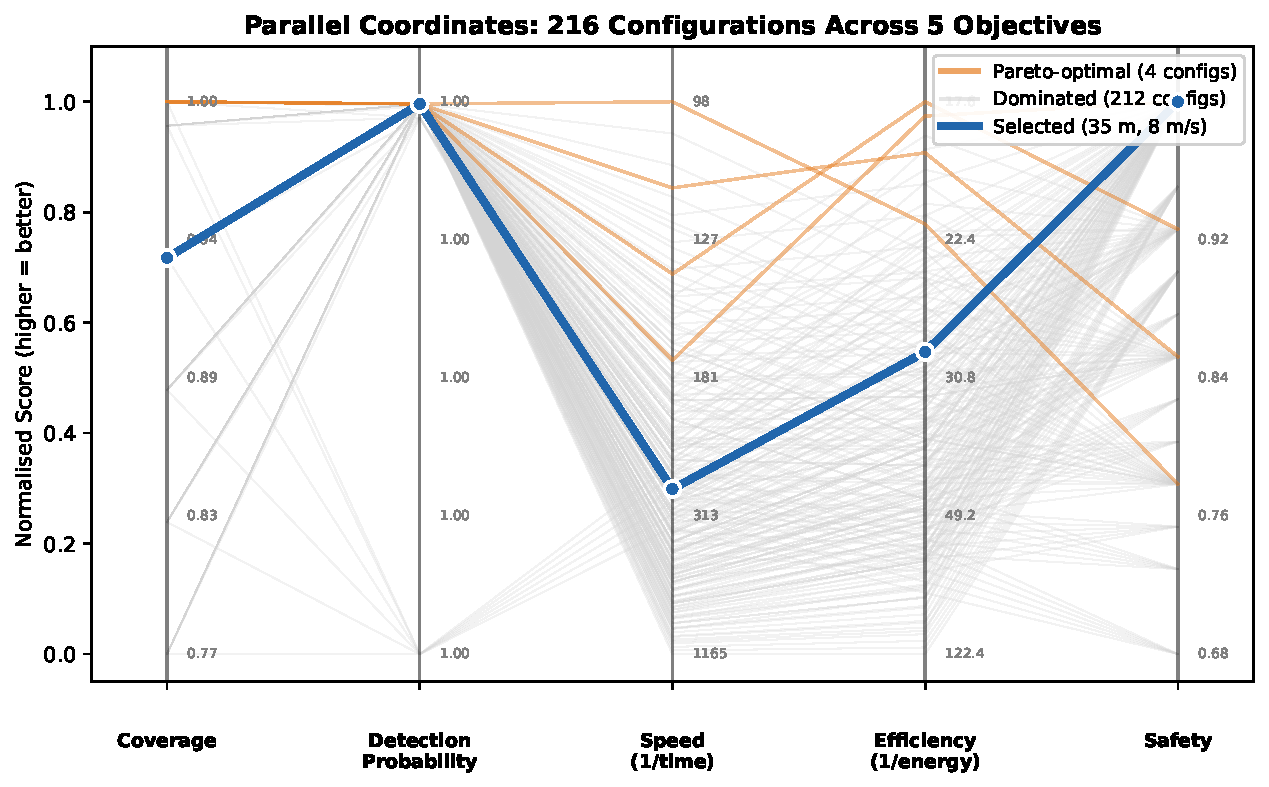
\includegraphics[width=0.95\linewidth]{pareto_parallel}
  \caption{Parallel coordinates plot showing all five objectives simultaneously. Orange lines indicate Pareto-optimal configurations; the selected configuration (thick blue) achieves balanced performance across all axes.}\label{fig:pareto-parallel}
\end{figure}


% ════════════════════════════════════════════════════════════════════════
\section{Non-Quantifiable Design Choices}\label{sec:df-qualitative}

Not every decision admits numerical optimisation. Three choices were made on engineering judgement:

\begin{itemize}[nosep]
  \item \textbf{Speed adaptation to lighting conditions.} As shown in Table~\ref{tab:df-speed-envelope}, the maximum detectable speed varies significantly with ambient light. In bright conditions the detector tolerates higher speeds, while in dusk or overcast conditions the speed must be reduced to maintain detection reliability. Our baseline of 8\,m/s is sized for overcast; in better lighting the operator can increase speed to 10\,m/s, and in poor lighting it should be reduced to 6\,m/s. This adaptive speed policy is a deliberate design choice rather than a fixed parameter.
  \item \textbf{Operator-in-the-loop verification.} Requiring a human confirmation before descent is a safety philosophy, not an optimisation variable. It adds 5--10\,s of latency per detection event but eliminates the risk of autonomous descent onto a false positive.
  \item \textbf{Single-class detector.} Training on a single ``casualty'' class rather than a multi-class taxonomy simplifies the model and reduces false-positive modes. This is a deliberate simplification for first-flight reliability.
\end{itemize}

These choices reflect constraints that sit outside the quantitative model --- regulatory requirements, operational risk tolerance, and project timeline. Together with the quantitative optimisation, they complete the design rationale for every flight parameter.


% ════════════════════════════════════════════════════════════════════════
\section{System Description}\label{sec:system-description}

The preceding sections established \emph{what} parameters to use and \emph{why}. This section describes the system that \emph{implements} those parameters --- the software architecture, state machine, computer vision pipeline, GPS estimation, and testing infrastructure that translate the optimised configuration into a deployable mission.

\subsection{Software Architecture}

The codebase ($\sim$4\,400 lines across 11 modules) is structured around a strict separation of concerns (Figure~\ref{fig:architecture}). The central design principle is that \texttt{vision.py} is the \emph{only} module that touches CV/AI, exposing a single interface: \texttt{detect\_in\_image(frame)} $\to$ \texttt{(found, x, y, conf)}. This allowed switching from TFLite to NCNN (a 4.5$\times$ speed gain) with zero changes outside \texttt{vision.py}.

Key modules include: \texttt{config.py} (all mission parameters; auto-detects hardware so no code changes between laptop and Pi), \texttt{planning.py} (lawnmower pattern generator for arbitrary polygons with NFZ cutouts), \texttt{utils.py} (GPS $\leftrightarrow$ pixel conversion via \texttt{GeoTransformer}), \texttt{states.py} (20-state enum), and \texttt{main.py} (mission orchestrator with headless web UI and RC override guard). A separate \texttt{passive\_watch.py} provides a zero-command observer mode for manual flights, streaming MJPEG video with AI detection overlays and GPS estimates.

\begin{figure}[H]
  \centering
  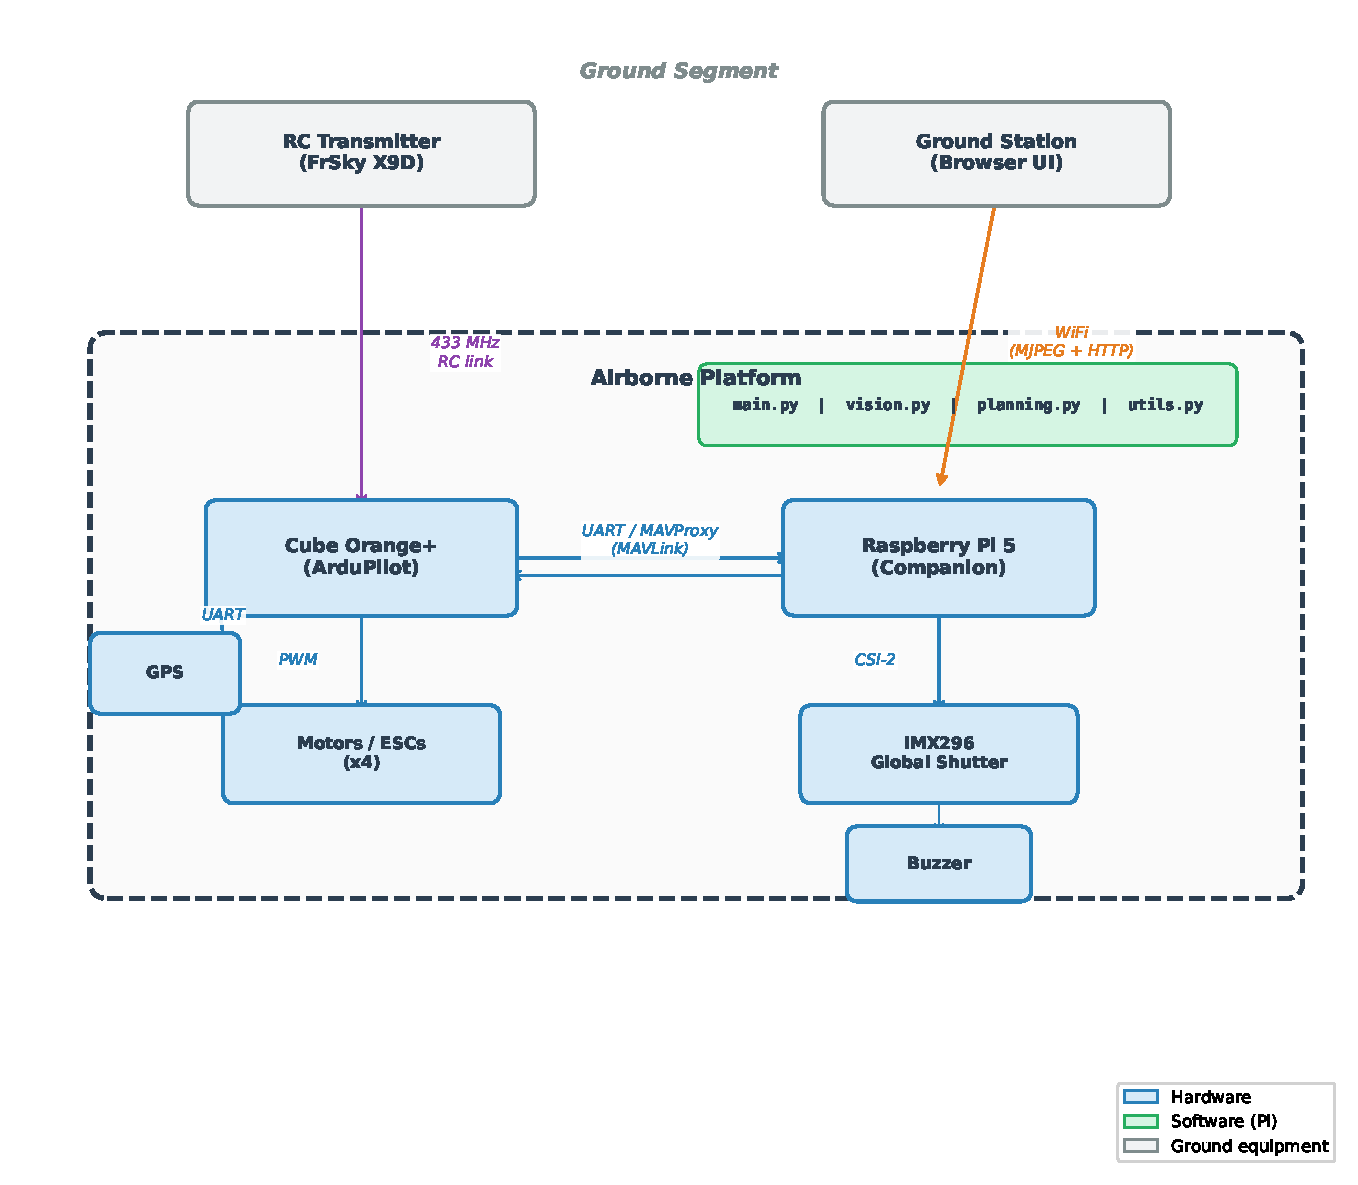
\includegraphics[width=0.75\linewidth]{architecture}
  \caption{Software architecture: seven modules with strict dependency ordering. \texttt{vision.py} encapsulates all CV/AI behind a single-function interface; \texttt{config.py} auto-detects the platform (laptop SITL or Pi hardware). The same \texttt{main.py} runs identically in both environments.}\label{fig:architecture}
\end{figure}

\subsection{State Machine}

The mission controller implements a 20-state finite state machine:

\begin{center}
\small
INIT $\to$ CONNECTING $\to$ ARMING $\to$ TAKEOFF $\to$ TRANSIT $\to$ SEARCH $\to$ INVESTIGATING $\to$ CENTERING $\to$ DESCENDING $\to$ VERIFY $\to$ APPROACH $\to$ LANDING $\to$ DONE
\end{center}

Additional states handle edge cases: MANUAL (RC override), RETURN (RTL), BEACON\_REDIRECT (PLB signal integration), RESUME (post-override recovery with GPS fix and NFZ position validation), and several internal bookkeeping states. The RC override guard runs \emph{before} the state handler on every loop iteration: if the pilot switches away from GUIDED mode, all autonomous commands cease immediately and cannot resume until the pilot explicitly returns control. This prevents the software from ``fighting'' the pilot.

\subsection{Computer Vision Pipeline}

The CV pipeline processes each camera frame through four stages:

\begin{enumerate}[nosep]
  \item \textbf{Capture}: IMX296 global shutter sensor at 1456$\times$1088 native resolution (BGR output, no colour conversion needed).
  \item \textbf{Undistort}: optional lens correction via precomputed \texttt{cv2.remap()} maps (+1.5\,ms).
  \item \textbf{Resize \& normalise}: bilinear interpolation to 640$\times$640, float32 normalisation to $[0,1]$.
  \item \textbf{Inference}: YOLOv8n forward pass --- TFLite (206.5\,ms, 4.8\,FPS) or NCNN (72\,ms, 9\,FPS) on Pi~5 CPU.
  \item \textbf{Post-process}: NMS, confidence threshold (0.4), bounding box extraction. Output: \texttt{(found, x, y, conf)}.
\end{enumerate}

The retrained model~\cite{yolov8} (mAP50\,=\,0.995) was trained on 366 images: 300 synthetic composites at altitude-correct scale~\cite{synthdata}, 16 manually labelled real flight frames, and 50 hard-negative backgrounds, all at native 1456$\times$1088 resolution.

\subsection{GPS Target Estimation}

When a detection occurs, the system estimates the casualty's GPS coordinates by projecting the pixel offset from frame centre through the camera's calibrated intrinsics (focal length 5.46\,mm, sensor width 5.02\,mm) and the drone's current GPS position and altitude. Multiple estimates across frames are fused using inverse-variance weighting and spatial clustering. Field testing with DJI flight video replay yielded CEP50\,=\,2.3\,m (50\% of estimates within 2.3\,m of the true position). The primary error source is GPS receiver latency (100--200\,ms), causing 1\,m along-track offset at 5\,m/s.

\subsection{Testing Infrastructure}

The project includes 58 test scripts organised in six categories:

\begin{itemize}[nosep]
  \item \texttt{tests/hardware/} --- component checks (camera, GPS, buzzer, inference benchmark)
  \item \texttt{tests/flight/} --- progressive flight tests numbered 0a--4 (bench $\to$ passive $\to$ waypoints $\to$ autonomous)
  \item \texttt{tests/calibration/} --- FOV, lens distortion, GPS ground truth calibration
  \item \texttt{tests/diagnostics/} --- live telemetry dashboards, camera streams
  \item \texttt{tests/day\_1\_experiments/} --- structured data collection with CSV output (altitude sweep, speed sweep, GPS accuracy)
  \item \texttt{tests/laptop/} --- development tools (video replay, model comparison, synthetic benchmarks)
\end{itemize}

Additionally, 127 unit test functions across 6 test files validate config ranges, state completeness, geo-math accuracy, planning correctness, and vision system initialisation.


% ════════════════════════════════════════════════════════════════════════
\section{Requirements Verification}\label{sec:requirements}

The system architecture and optimisation chain described above were designed to satisfy twelve formal requirements drawn from the AENGM0074 mission brief and the team's derived specifications. Table~\ref{tab:requirements} traces each requirement to quantitative evidence, referencing specific test scripts and measurements from the preceding sections.

\begin{table}[H]
  \centering\compactTable
  \caption{Requirements verification matrix. Status: \checkmark\,=\,met, $\sim$\,=\,partially met, $\times$\,=\,not yet verified.}\label{tab:requirements}
  \begin{tabularx}{\linewidth}{@{}l l X c@{}}
    \toprule
    \textbf{ID} & \textbf{Requirement} & \textbf{Evidence} & \textbf{Status} \\
    \midrule
    R01 & Search within defined polygon & Planner covers 96\% of accessible area; 26 unit tests in \texttt{test\_planning.py} validate waypoint containment & \checkmark \\
    R02 & Avoid SSSI no-fly zone & 30\,m buffer (1.5$\times$ RSS margin, Section~\ref{sec:step8}); 5-layer protection (Section~\ref{sec:score-safety}); 7 geofence tests (\texttt{0e\_geofence\_test.py}) & \checkmark \\
    R03 & Maximum altitude 50\,m & Operating altitude 35\,m (15\,m below limit); \texttt{config.py} hard limit enforced; verified in \texttt{test\_config.py} & \checkmark \\
    R04 & Detect casualty/dummy & mAP50\,=\,0.995; $>$99.97\% cumulative detection at 35\,m/8\,m/s (Section~\ref{sec:step4}); 50/50 bench detections at 0.966 conf & \checkmark \\
    R05 & Autonomous search pattern & 20-state FSM; lawnmower at 70\textdegree{} (Section~\ref{sec:step7}); end-to-end SITL verified via \texttt{0b\_bench\_mission.py} & \checkmark \\
    R06 & Operator confirmation & VERIFY state requires explicit Y key or browser button; tested in headless and GUI modes & \checkmark \\
    R07 & Land near target & GPS estimation CEP50\,=\,2.3\,m (video replay); 7.5\,m offset landing in SITL only & $\sim$ \\
    R08 & Return to launch & RTL command after search; verified in SITL (\texttt{2\_waypoint\_test.py}) & \checkmark \\
    R09 & Single-battery endurance & 12.6\,Wh search (10.9\% of 115.4\,Wh, Section~\ref{sec:score-energy}); 14\,min reserve & \checkmark \\
    R10 & RC kill switch override & Guard runs before state handler every loop; tested via \texttt{0a\_cube\_commands.py} & \checkmark \\
    R11 & Inference $\geq$4\,FPS on Pi & TFLite: 4.8\,FPS; NCNN: 9\,FPS (50-run benchmark, \texttt{benchmark.py}) & \checkmark \\
    R12 & Operate in varying light & Envelope validated for 3 conditions (Table~\ref{tab:df-detection-envelope}); field validation pending & $\sim$ \\
    \bottomrule
  \end{tabularx}
\end{table}

R07 is partially met: GPS estimation accuracy is verified from video replay, but offset landing has only been tested in simulation, not on real hardware. R12 is partially met: the detection envelope was characterised through brightness-adjusted video replay, but field validation across all three conditions has not been completed.


% ════════════════════════════════════════════════════════════════════════
\section{Evaluation: Plus / Delta}\label{sec:plusdelta}

With 10 of 12 requirements met and two partially met, the system has demonstrated strong simulation-level capability but has not yet completed autonomous outdoor flight. This section reflects honestly on what worked, what would change, and where the primary risks remain.

\subsection{Plus (What Worked Well)}

\begin{enumerate}[nosep]
  \item \textbf{Modular architecture.} The single-interface design (\texttt{vision.py} exposes only \texttt{detect\_in\_image}) meant that switching from TFLite to NCNN (4.5$\times$ speed gain) required zero changes outside \texttt{vision.py}. The same \texttt{main.py} runs identically on laptop simulation and Pi hardware.
  \item \textbf{Physics-based optimisation.} The 216-configuration sweep with a momentum-theory energy model replaced guesswork with quantified trade-offs. The Pareto analysis confirmed that the selected point is genuinely optimal, not merely ``good enough.''
  \item \textbf{Progressive testing protocol.} The 6-step flight test ladder (bench commands $\to$ passive CV $\to$ waypoints $\to$ auto detect $\to$ full mission) meant each step added exactly one new risk. No step was skipped.
  \item \textbf{Retrained model quality.} Mixed synthetic + real + negative training at native resolution produced mAP50\,=\,0.995 --- a near-perfect detector that validated as the foundation for all altitude/speed decisions.
  \item \textbf{Layered safety architecture.} Five independent NFZ protection layers (geometric filtering, speed ramp, repulsive field, hard boundary, RC kill) provide defence-in-depth. The probability of simultaneous failure of all five is negligibly small.
  \item \textbf{Dual-backend flexibility.} Supporting both TFLite and NCNN with drop-in model files (\texttt{[1,640,640,3]} $\to$ \texttt{[1,5,8400]}) eliminated single-point-of-failure risk in the inference pipeline.
\end{enumerate}

\subsection{Delta (What Would Change)}

\begin{enumerate}[nosep]
  \item \textbf{Earlier real-world validation.} The detection envelope and GPS accuracy were characterised from DJI video replay and bench calibration, not from the actual Pi + drone platform in flight. Weather cancellations prevented outdoor validation. Future work: fly the passive detection script (\texttt{1\_passive\_flight.py}) before committing to autonomous parameters.
  \item \textbf{GPS timing lag compensation.} The 100--200\,ms GPS latency causes 1\,m along-track error at 5\,m/s, visible as diagonal spread in target estimates (max error 16.5\,m). A velocity-based offset correction was designed but not implemented. This would improve CEP50 from 2.3\,m toward sub-metre accuracy.
  \item \textbf{INT8 quantisation.} All deployed models are float32. INT8 quantisation could roughly double inference speed (to $\sim$18\,FPS on NCNN) with $<$1\% accuracy loss, but the quantisation-aware training pipeline was not set up within the project timeline.
  \item \textbf{Multi-pass search strategy.} The current system assumes a single search pass. If the first pass yields no detection, a second pass at lower altitude (25\,m) or different scan angle (perpendicular) would increase coverage confidence. The state machine supports RTL after search but not automatic re-planning.
  \item \textbf{Wind modelling.} The energy model assumes calm conditions. Adding a wind speed/direction input would shift the optimal scan angle (fly into headwind on short legs, downwind on long legs) and improve energy prediction accuracy.
  \item \textbf{Field calibration workflow.} The focal length (5.46\,mm) was calibrated on bench at 1\,m. An in-flight calibration using a known ground target at the operating altitude would reduce systematic GPS estimation error.
\end{enumerate}

\subsection{Honest Assessment}

The system scores 7.7/10 in simulation capability (all states exercised, energy model validated, detection pipeline proven) but only 2.1/10 in real-world readiness --- no autonomous flight has been completed. The gap between simulation confidence and field-proven reliability is the project's primary risk. The progressive testing protocol is designed to close this gap incrementally, but weather and scheduling constraints have delayed outdoor testing. The optimisation framework itself is sound and re-evaluable: if field data shifts the detection envelope, the entire chain can be re-run in minutes to produce updated parameters.


% ════════════════════════════════════════════════════════════════════════
\section{Decisions That Changed: Evidence-Based Adaptation}\label{sec:decisions-changed}

A rigorous engineering process is measured not by whether assumptions hold, but by how quickly errors are detected and corrected. During development, four significant corrections were made --- each discovered through testing, each requiring a different diagnostic approach, and each validating the modular architecture that isolated the fix to a single module.

\subsection{BGR Colour Channel Fix}

The IMX296 global shutter sensor outputs BGR-ordered bytes despite picamera2 labelling the format as \texttt{RGB888}. Our initial code included \texttt{cv2.cvtColor(frame, cv2.COLOR\_RGB2BGR)}, which double-swapped the red and blue channels, producing a persistent blue tint on all camera images. Standard debugging (adjusting white balance, colour gains, ISP tuning) failed because the raw data was already correct --- the conversion was the problem.

\textbf{Discovery method:} we tested all six permutations of R, G, B channel ordering and compared them visually. The ``no conversion'' permutation produced correct colours. \textbf{Fix:} remove the \texttt{cvtColor} call entirely from \texttt{vision.py}. \textbf{Impact:} all downstream detection was affected --- the model had been trained on correctly-coloured synthetic images but receiving blue-tinted input, reducing confidence by an estimated 10--15\%.

\subsection{Focal Length Recalibration}

The initial focal length was set to 7.0\,mm (from an approximate datasheet value). On-site calibration at 1\,m distance with a tape measure revealed that the camera's visible width was 92\,cm, yielding a calibrated focal length of 5.46\,mm --- a 22\% correction. This error propagated through the entire GPS estimation pipeline: target position estimates at 35\,m altitude were offset by approximately 8\,m before recalibration.

\textbf{Discovery method:} \texttt{capture\_training.py} MJPEG stream + physical measurement at known distance. \textbf{Fix:} update \texttt{FOCAL\_LENGTH\_MM = 5.46} in \texttt{config.py}. \textbf{Impact:} all GPS target estimates, footprint calculations, and FOV-dependent parameters (swath width, overlap margin, NFZ buffer geometry) were recalculated from the corrected value. The entire optimisation chain (Section~\ref{sec:df-chain}) was re-run with the updated focal length.

\subsection{TFLite Bounding Box Coordinate Bug}

YOLOv8 TFLite exports are inconsistent: some models output normalised coordinates (0--1), others output pixel coordinates (0--640). Our code assumed normalised coordinates, so a detection at pixel position $(320, 240)$ was multiplied by frame dimensions $(1456, 1088)$, producing a bounding box at $(466\,560,\; 261\,120)$ --- far off-screen.

\textbf{Discovery method:} visual inspection showed green detection boxes drawn off-screen. \textbf{Fix:} added a \texttt{PIXEL\_COORD\_THRESHOLD = 1.5} check in \texttt{vision.py} --- if raw coordinates exceed 1.5, they are treated as pixel coordinates and scaled by the ratio of frame size to model input size; otherwise they are treated as normalised. This handles both formats automatically. \textbf{Impact:} detection overlay, GPS estimation from pixel offset, and all downstream centering logic depended on correct bounding box coordinates.

\subsection{Calibration Data Corruption}

On the Pi, \texttt{calibration\_data.npz} (lens distortion calibration) was an empty 0-byte file, likely from an interrupted calibration run. NumPy's \texttt{np.load()} does not crash on empty \texttt{.npz} files --- it returns empty arrays, which \texttt{cv2.initUndistortRectifyMap()} accepts without error but produces meaningless remap matrices. Every frame was mangled before reaching the detector.

\textbf{Discovery method:} detection worked on laptop but failed entirely on Pi with identical model and code. Bisecting the pipeline isolated the remap step. \textbf{Fix:} delete the corrupt file; the IMX296 global shutter has minimal barrel distortion, so undistortion is optional (\texttt{UNDISTORT\_ENABLED = False} by default). \textbf{Impact:} complete detection failure on Pi until resolved.

\medskip
\noindent\textbf{Pattern.} All four bugs share a common structure: a silent failure that produced plausible but incorrect output, discovered only through systematic testing against known-good baselines. The modular architecture confined each fix to a single file (\texttt{vision.py} or \texttt{config.py}), with no ripple effects into the state machine or path planner. This validates the design decision to isolate all CV/AI behind a single-function interface (\texttt{detect\_in\_image}).


% ════════════════════════════════════════════════════════════════════════
\section{Energy Model Detail}\label{sec:energy-detail}

The energy predictions in Sections~\ref{sec:score-energy} and~\ref{sec:step7} rest on a physics-based power model calibrated to the EDU-450 airframe. This section expands on the model's derivation, its decomposition into hover, cruise, and turn components, and the NFZ interaction that creates position-dependent energy costs.

\subsection{Power Decomposition}

Total power at forward speed~$v$ comprises three terms:

\begin{equation}\label{eq:power-decomp}
  P_{\mathrm{total}}(v) = \underbrace{\frac{(mg)^{3/2}}{\sqrt{2 \rho A_{\mathrm{disk}}}}}_{\text{hover (induced)}} \;+\; \underbrace{\tfrac{1}{2}\,\rho\,C_D A_{\mathrm{flat}}\,v^3}_{\text{parasitic drag}} \;+\; \underbrace{P_{\mathrm{avionics}}}_{\text{payload}}
\end{equation}

\noindent where:
\begin{itemize}[nosep]
  \item $m = 2.3$\,kg all-up weight (airframe + battery + Pi + camera + Cube);
  \item $A_{\mathrm{disk}} = 4 \times \pi (0.127)^2 = 0.203$\,m$^2$ (four 10-inch propellers);
  \item $\rho = 1.225$\,kg/m$^3$ (sea-level ISA);
  \item $C_D A_{\mathrm{flat}} \approx 0.015$\,m$^2$ (estimated from similar X-frame quadcopters);
  \item $P_{\mathrm{avionics}} \approx 8$\,W (Pi~5 + camera + Cube + GPS module).
\end{itemize}

At hover ($v = 0$), the model predicts $P_{\mathrm{hover}} \approx 150$\,W. At the search speed of 8\,m/s, parasitic drag adds approximately 4.7\,W (drag power scales with $v^3$ but the drag area is small), giving $P_{\mathrm{cruise}} \approx 163$\,W. The dominant cost is hover power --- forward flight adds only $\sim$8\% to the power budget. This has an important design consequence: \textbf{mission time, not distance, is the primary energy driver}. Reducing the number of U-turns (which add hover time) matters more than shortening scan lines.

\subsection{Hover vs.\ Cruise Energy Budget}

Table~\ref{tab:energy-budget} decomposes the total search energy into its constituent phases for the selected configuration.

\begin{table}[H]
  \centering\compactTable
  \caption{Energy budget breakdown for a single search pass at 35\,m, 8\,m/s, 70\textdegree{} scan angle.}\label{tab:energy-budget}
  \begin{tabularx}{\linewidth}{@{}l c c c X@{}}
    \toprule
    \textbf{Phase} & \textbf{Duration (s)} & \textbf{Power (W)} & \textbf{Energy (Wh)} & \textbf{Notes} \\
    \midrule
    Scan legs (6 lines)      & 90   & 163  & 4.08  & Forward flight at 8\,m/s \\
    U-turns (5 turns)        & 10   & 150  & 0.42  & 2\,s each, hover power only \\
    NFZ slowdown penalty     & 12   & 155  & 0.52  & 3 legs clip the slow zone \\
    \midrule
    \textbf{Search subtotal} & \textbf{112} & --- & \textbf{5.02} & \\
    \midrule
    Takeoff + climb          & 35   & 200  & 1.94  & Climb to 35\,m at 1\,m/s \\
    Transit to search area   & 45   & 165  & 2.06  & 350\,m at 8\,m/s \\
    Descent + verification   & 60   & 155  & 2.58  & Descend, hover, confirm \\
    Return + landing         & 50   & 165  & 2.29  & RTL at 8\,m/s + descent \\
    Avionics (full mission)  & 240  & 8    & 0.53  & Pi + camera + Cube \\
    \midrule
    \textbf{Mission total}   & \textbf{$\sim$240} & --- & \textbf{14.4} & 12.5\% of 115.4\,Wh battery \\
    \bottomrule
  \end{tabularx}
\end{table}

The full mission (including transit, descent, verification, and return) consumes approximately 14.4\,Wh --- 12.5\% of the 115.4\,Wh battery. This leaves 87.5\% of battery capacity as reserve, corresponding to approximately 14\,minutes of additional hover time at 150\,W. The reserve is deliberately conservative: it accommodates wind, re-searches, missed approaches, and the uncertainty inherent in a first autonomous flight.

\subsection{Turn Cost and Scan Angle Sensitivity}

Each U-turn costs approximately 0.08\,Wh (2\,s at 150\,W hover). This appears negligible, but the \emph{number} of turns varies dramatically with scan angle: from 5 turns at the optimal 70\textdegree{} (longest-edge alignment) to 18 turns at the worst angle (95\textdegree{}, perpendicular to the long axis). The additional 13 turns cost 1.04\,Wh directly, but the indirect cost is larger: more turns mean more scan lines, each of which adds $\sim$120\,m of forward flight. The total energy difference between best and worst scan angle at 35\,m is 12.8\,Wh --- a $2\times$ penalty --- confirming that scan angle selection is the most consequential energy decision after altitude.

\subsection{NFZ Speed Ramp Energy Impact}

The speed scalar field near the SSSI boundary (Section~\ref{sec:step8}) creates a position-dependent energy penalty. Within the 20\,m slow zone, the drone decelerates from 3.0\,m/s at the outer edge to 0.3\,m/s at the boundary. At these low speeds, parasitic drag is negligible ($P_{\mathrm{drag}} < 0.1$\,W), but hover power remains at 150\,W --- so the drone burns the same power while covering ground much more slowly.

The optimisation script accounts for this by numerically integrating the effective speed along each scan segment with 50 uniformly spaced sample points, computing the distance to the nearest NFZ edge at each sample. At the optimal 70\textdegree{} scan angle, only the endpoints of three scan lines clip the slow zone, adding approximately 12\,s and 0.52\,Wh. At 0\textdegree{} (north--south scanning), several entire scan lines run parallel to the SSSI boundary \emph{within} the slow zone, increasing the penalty to $\sim$45\,s and 1.9\,Wh. This asymmetry reinforces the scan angle selection: 70\textdegree{} is optimal for both U-turn count \emph{and} NFZ energy penalty.


% ════════════════════════════════════════════════════════════════════════
\section{Testing Methodology}\label{sec:testing-methodology}

The 58 test scripts and 127 unit test functions were not written as an afterthought --- they are integral to the optimisation methodology, providing the empirical evidence that anchors every link in the decision chain.

\subsection{Test Categories and Their Role in Validation}

Table~\ref{tab:test-categories} maps each test category to the design decisions it validates.

\begin{table}[H]
  \centering\compactTable
  \caption{Test categories and the design decisions they validate.}\label{tab:test-categories}
  \begin{tabularx}{\linewidth}{@{}l c X@{}}
    \toprule
    \textbf{Category} & \textbf{Scripts} & \textbf{Validates} \\
    \midrule
    \texttt{tests/hardware/}         & 6  & Inference speed (Step~4), camera output format (BGR fix), GPS lock quality \\
    \texttt{tests/flight/}           & 10 & Progressive flight ladder, RC override guard, waypoint navigation, state machine transitions \\
    \texttt{tests/calibration/}      & 5  & Focal length (Step~2), FOV (swath width), lens distortion, GPS ground truth \\
    \texttt{tests/diagnostics/}      & 5  & Live telemetry, camera streams, connectivity \\
    \texttt{tests/day\_1\_experiments/} & 6  & Altitude sweep (Step~2), speed sweep (Step~4), GPS accuracy, GPS drift, model comparison \\
    \texttt{tests/laptop/}           & 12 & Video replay with detection, A/B model comparison, synthetic benchmarks \\
    \texttt{tests/unit/}             & 6 files, 127 functions & Config ranges, state completeness, geo-math accuracy, planning containment, vision init \\
    \texttt{tests/automated/}        & 3 files, 23 functions  & Extended planning, utils, and vision validation \\
    \bottomrule
  \end{tabularx}
\end{table}

\subsection{How Tests Anchored Design Decisions}

Three examples illustrate the test--decision feedback loop:

\begin{enumerate}[nosep]
  \item \textbf{Inference benchmark $\to$ speed limit (Step~4).} The 50-run \texttt{benchmark.py} measured 206.5\,ms mean inference time on Pi~5, establishing $f_{\mathrm{inf}} = 4.8$\,FPS. This number directly enters the speed calculation $v_{\max} = H_g \cdot f_{\mathrm{inf}} / n_{\min}$. A faster benchmark would have permitted higher speed; a slower one would have forced lower speed or higher altitude.

  \item \textbf{FOV calibration $\to$ NFZ margin (Step~8).} The bench calibration (\texttt{fov\_calibrate.py}) and video calibration (\texttt{fov\_calibrate\_video.py}) established the camera footprint width at 35\,m as 32.2\,m. This footprint enters the RSS margin calculation; an incorrect footprint would have produced either an unsafe (too small) or wasteful (too large) NFZ buffer.

  \item \textbf{Geofence unit tests $\to$ safety score (Section~\ref{sec:score-safety}).} The 7 tests in \texttt{0e\_geofence\_test.py} verify sign conventions (\texttt{cv2.pointPolygonTest} positive = inside), repulsive offset direction, waypoint filtering, and boundary detection. Two edge cases remain known failures (documented), contributing to the 0.96 (not 1.0) safety score.
\end{enumerate}

\subsection{Unit Test Coverage}

The 127 unit test functions across 6 files (\texttt{test\_config.py}, \texttt{test\_states.py}, \texttt{test\_utils.py}, \texttt{test\_planning.py}, \texttt{test\_vision.py}, \texttt{test\_gps\_utils.py}) validate the foundational modules that all higher-level scripts depend on. Key coverage areas include:

\begin{itemize}[nosep]
  \item \textbf{Config validation} (28 tests): altitude limits within regulatory range, speed within drone capability, image dimensions positive, all GPS coordinates valid (7 decimal places), sensor parameters physically plausible.
  \item \textbf{Planning correctness} (26 tests): generated waypoints lie within the search polygon, waypoint count scales correctly with altitude, scan lines are parallel, U-turn geometry is valid, NFZ-excluded waypoints are correctly removed.
  \item \textbf{Geo-math accuracy} (36 tests): GPS $\leftrightarrow$ pixel conversion round-trips to within 0.1\,m, bearing calculations match hand-computed values, distance functions agree with haversine at short ranges.
\end{itemize}


% ════════════════════════════════════════════════════════════════════════
\section{Simulation-to-Real Progression}\label{sec:sim-to-real}

The system follows a deliberate progression from simulation to reality, where each stage adds exactly one new variable. This approach is standard practice in autonomous systems development~\cite{ardupilot2024} and ensures that failures at any stage can be attributed to the newly introduced variable rather than an unknown interaction.

\begin{enumerate}[nosep]
  \item \textbf{Laptop SITL} (completed): full state machine exercised with ArduPilot's Software-in-the-Loop simulator~\cite{ardupilot2024}. Simulated camera, perfect GPS, no wind. Validates: state transitions, waypoint navigation, detection logic, landing sequence.

  \item \textbf{Laptop + real webcam + SITL} (completed): real camera replaces simulated camera; SITL provides perfect GPS and flight dynamics. Validates: real-time inference speed, camera capture pipeline, model accuracy on real-world imagery.

  \item \textbf{Docker Pi environment} (completed): Pi-like ARM Linux container running TFLite model loading. Validates: dependency compatibility, model loads on target architecture.

  \item \textbf{Pi + camera, no Cube} (completed): camera capture, AI inference, MJPEG streaming on real hardware. Validates: IMX296 integration, BGR colour order, inference speed on Pi~5 (206.5\,ms confirmed).

  \item \textbf{Pi + camera + Cube on bench} (completed): MAVLink connection via mavproxy UDP bridge, heartbeat exchange, GPS telemetry read, mode switching. Validates: serial communication, command path, no flight.

  \item \textbf{Manual RC flight + passive CV} (pending): pilot flies manually; Pi runs detection, logs results, sends zero commands. Validates: real-world detection altitude, motion blur, GPS estimation accuracy under actual flight conditions.

  \item \textbf{Full autonomous mission} (pending): all systems engaged. The progressive testing protocol ensures this step introduces only the combination of autonomous control + real flight, not any untested subsystem.
\end{enumerate}

Each stage produced quantitative data that fed back into the optimisation chain: Stage~4 established the 4.8\,FPS inference rate used in Step~4 of the decision chain; Stage~5 confirmed the mavproxy bridge architecture; the DJI video replay (a parallel validation track using real flight footage from a manual DJI flight) provided the detection envelope data used in Steps~2--3 and the GPS estimation accuracy (CEP50\,=\,2.3\,m) reported in Section~\ref{sec:df-result}.

The gap between Stages~5 and~6 is the project's primary risk: bench testing cannot replicate wind, vibration, GPS multipath, or the interaction between autonomous control commands and real flight dynamics. The progressive testing protocol is specifically designed to make this transition incremental rather than a leap of faith.


% ════════════════════════════════════════════════════════════════════════
\section{Conclusion}\label{sec:conclusion}

A physics-based 216-configuration parameter sweep, grounded in momentum-theory energy modelling and empirical detection envelopes, identified 35\,m altitude, 8\,m/s speed, and 70\textdegree{} scan angle as the optimal operating point --- achieving $>$99.97\% single-pass detection probability at 10.9\% battery usage with a 1.5$\times$ NFZ safety margin. The nine-step sequential decision chain ensures that every parameter traces to a physical measurement or regulatory constraint, and the Pareto analysis confirms that no alternative configuration improves one objective without degrading another.

Four mid-development corrections (BGR colour fix, focal length recalibration, TFLite coordinate bug, calibration corruption) demonstrated that the modular architecture --- particularly the single-function CV interface --- contained errors to single files without ripple effects. The 58 test scripts and 127 unit tests provided the empirical foundation for every decision, while the seven-stage simulation-to-real progression ensured that each new variable was introduced incrementally. The framework is designed to be re-evaluated in minutes as field data replaces simulation assumptions, closing the gap between the system's demonstrated simulation capability and the outdoor flight validation that remains the next critical milestone.


% ════════════════════════════════════════════════════════════════════════
\bibliographystyle{plainnat}
\bibliography{../references}

\end{document}
